% Imported from LaTeX_and_pdfs/DGDT_dump.tex; see provenance.json.
\part{Classical Mechanics}


\problemhead{1.4 The altitude angle of the Sun, Japan Physics Olympiad (2014)} cf. Japan Physics Olympiad, (2014) \cite{dgdt:Japa2014}.


\solutionhead{1.4 The altitude angle of the Sun, Japan Physics Olympiad (2014)}

\quad \\ 

$NC \equiv$ Niigata City, \\
$AM \equiv $ Amagi-san in Izu. \\

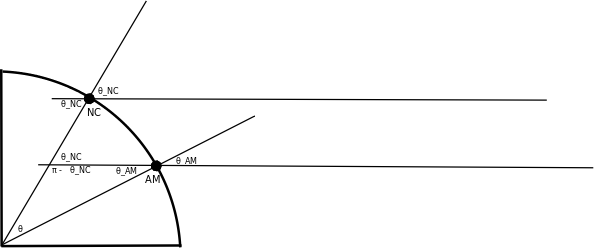
\includegraphics[scale=0.7]{./Prob1_4_altitude_angle_of_sun.png}

From all 3 internal angles of a triangle sum up to 180 degrees, or i.e. $\pi$ radians,
\[
\begin{gathered}
	\pi = \pi - \theta_{NC} + \theta_{AM} + \theta \Longrightarrow \boxed{ \theta = \theta_{NC} - \theta_{AM}} 
\end{gathered}
\]
So we've shown indeed that $\theta$ is the \textbf{difference between altitude angles of the Sun} at NC and AM, respectively.


From 
\[
\begin{gathered}
\begin{aligned}
	& C = 2 \pi R \\
 	& l_M = \theta R 
\end{aligned} \\
\frac{ l_M }{l} = \frac{ \theta R}{  \frac{\pi}{2} R } \text{or } \frac{ l_M}{l} = \frac{ 2 \theta}{ \pi} \\
 \Longrightarrow \theta = \frac{\pi}{2} \frac{ l_M}{l} = \frac{\pi}{2} \cdot \frac{334 \times 10^3 \, m}{ 10^7 m} \cdot \frac{ 180^{\circ} }{ \pi} = 3^{\circ}
\end{gathered}
\]

Advice, remember to draw a \emph{cross-section} to make diagram clear, rather than worry about "the other transverse dimension". Also, draw the lines literally parallel to the Sun because of how far away the Sun is and how large the Sun is.


\section{Structure of Galilean Space-Time}

cf. Sec. 3.1 - \emph{Structure of Galilean Space-Time} of Pr\'{a}staro (1996) \cite{dgdt:Pras1996}.

Mechanics assumes a particular simple formulation if formulated with respect to some spacetime manifold.

In Galilean spacetime, it's possible to naturally recognize absolute objects, and others that depend on frames.

cf. Def. 3.1 of Pr\'{a}staro (1996) \cite{dgdt:Pras1996}
\begin{definition}[Galilean spacetime structure]
\begin{enumerate}
	\item Galilean spacetime structure $:= (\mathcal{G}, g)$ where \\
	$\mathcal{G}$ is (fiber bundle space-time)
	\begin{equation}
		\mathcal{G} \equiv \lbrace \tau : M \to T \rbrace
	\end{equation}
	where \\
	$M = $ 4-dim. affine manifold (\textbf{space-time}); corresponding structure is $(M, \mathbf{M}, \alpha)$, \\
\item	$T = $ 1-dim. affine space (\textbf{time}), corresponding affine structure is $(T, \mathbf{T}, \beta)$
\item $\tau = $ surjective affine mapping, of constant rank $1$, s.t. $\forall \, p \in M$ associates its time $\tau(p) \in T$
\end{enumerate}

Put $\mathbf{S} = \text{ker}(\underline{\tau}) \equiv \text{ker}(D\tau)\in M$, \\
	where $\underline{\tau} \equiv D\tau$, $D$ is symbol of derivative.\\	
	Define 
	\[
	\begin{aligned}
	& g: M \to vS_2^0(M) \equiv M \times S_2^0(\mathbf{S}) \\ 
	& g(p) = (p, \underline{g})  \equiv (p, Dg) , \forall \, p \in M
	\end{aligned}
	\]
	where $\underline{g} \equiv Dg$ is a Euclidean structure on $\mathbf{S}$.  $g$ is called vertical metric field.
\end{definition}

Thus, given $(M, \mathbf{M}, \alpha)$, $\forall \, (O, \lbrace \mathbf{e}_i)_{1 \leq i \leq d}$, $\lbrace \mathbf{e}_i \rbrace_{i=1\dots d}$, is basis of $\mathbf{M}$, 
\[
M \cong \mathbb{R}^4, \text{and } \exists \, \lbrace x^{\alpha} : M = \mathbb{R}^4 \to \mathbb{R} \rbrace_{\alpha = 1 \dots 4}
\]

cf. 1.1.3 Principle of Relativity, pp. 9, 1 Basic Principles of Classical Mechanics, Arnold, Kozlov, Neishtadt (2006) \cite{dgdt:AKN2006}.

direct product $E^3 \times \mathbb{R}\lbrace t \rbrace$ (spacetime) has natural structure of affine space \\
Galilean group is by def. group of all affine transformations of $E^3 \times \mathbb{R}$ that preserve time intervals and are isometries of space $E^3 \, \forall \,$ fixed $t\in \mathbb{R}$.  \\

Thus if 
\begin{definition}[Galilean group]\label{dgdt:Def:GalileanGroup}
\textbf{Galilean group} is group of all affine transformations of $E^3 \times \mathbb{R}$ that preserve time intervals and are isometries of space $E^3 \, \forall \, $ fixed $t\in \mathbb{R}$. \\

Thus, if Galilean transformation $g$, 
\begin{equation}
\begin{aligned}
& g: E^3 \times \mathbb{R}\lbrace t\rbrace \to E^3 \times \mathbb{R} \lbrace t \rbrace \\
& g:(s,t) \mapsto (s', t')
\end{aligned}
\end{equation}
\begin{enumerate}
	\item $t_{\alpha} - t_{\beta} = t'_{\alpha} - t'_{\beta}$ \\
	\item if $t_{\alpha} = t_{\beta}$, then $|s_{\alpha} - s_{\beta} | = |s'_{\alpha} - s_{\beta}' |$
\end{enumerate}

\end{definition}

Consider $(s_a,t_a), (s_b, t_b)$, $t_a - t_b$, $|s_a - s_b|$.
\[
\begin{gathered}
\begin{aligned}
	& g(s_a, t_a) = (s'_a, t'_a) \\ 
	& g(s_b,t_b) = (s'_b, t'_b)
\end{aligned} \\
\begin{aligned}
& t_a' - t'_b = \pi_tg(s_a, t_a) - \pi_tg(s_b, t_b) = t_a - t_b \\ 
& |s_a' - s'_b| = | \pi_s g(s_a,t_a) - \pi_sg(s_b,t_b) | = |s_a-s_b|
\end{aligned}
\end{gathered}
\]

Galilean group $g$ acts on $\mathbb{R}^3\lbrace \mathbb{r} \rbrace \times \mathbb{R} \lbrace t \rbrace$. \\

\subsection{3 examples of Galilean transformations}

uniform motion with constant velocity $\mathbf{v}$:
\begin{equation}
g_1(\mathbf{r}, t) = (\mathbf{r} + \mathbf{v} t, t)
\end{equation}

translation of origin in spacetime
\begin{equation}
g_2(\mathbf{r}, t) = (\mathbf{r} + \mathbf{x} , t + \alpha )
\end{equation}

rotation of coordinate axes
\begin{equation}
g_3(\mathbf{r}, t) = (G \mathbf{r}, t)
\end{equation}
where $G: \mathbb{R}^3 \to \mathbb{R}^3$ is orthonormal transformation.

\begin{proposition}[Galilean transformation decomposition]
	$\forall \, $ galilean transformation $g: \mathbb{R}^3 \times \mathbb{R} \to \mathbb{R}^3 \times \mathbb{R}$ can be uniquely represented as composition $g_1g_2 g_3$
\end{proposition}
cf. Prop. 1.1 of Arnold, Kozlov, Neishtadt (2006) \cite{dgdt:AKN2006} 

\begin{proof}
Consider affine transformation of $E^4 = E^3 \times \mathbb{R}$ of general form
\[
\begin{aligned}
& \mathbf{x} = A\mathbf{x}' + \mathbf{v} t' + \mathbf{a} \\ 
& t = \langle \mathbf{l} , \mathbf{x}' \rangle + kt' + s 
\end{aligned}
\]
$A \in \text{Mat}_{\mathbb{R}}(3,3)$, $\mathbf{v}, \mathbf{a}, \mathbf{l} \in \mathbb{R}^3$, $k, s \in \mathbb{R}$. \\


By galilean transformation (Def. \ref{dgdt:Def:GalileanGroup}), $t_2 - t_1 = t_2' - t_1'$, so 
\[
\begin{gathered}
t_2 - t_1 = \langle \mathbf{l} , \mathbf{x}'_2 \rangle + k t'_2 + s - \langle \mathbf{l}, \mathbf{x}'_1 \rangle - k t'_1 - s = \langle \mathbf{l}, \mathbf{x}'_2 - \mathbf{x}'_1 \rangle + k (t'_2 - t'_1) = t'_2 - t'_1
\end{gathered}\]
	
Since each of the 3 components of $\mathbf{x}_2 - \mathbf{x}_1$ are arbitrary, $\mathbf{l} = 0$, $k=1$ clearly. Or, let $t=2 = t_1$. Then clearly $\mathbf{l}=0$. \\

By galilean transformation (Def. \ref{dgdt:Def:GalileanGroup}), $|\mathbf{x}_2 - \mathbf{x}_1 | = |\mathbf{x}'_2 - \mathbf{x}'_1 |$ \\

Let $t_2 = t_1$. \\
\[
\begin{gathered}
|\mathbf{x}_2 - \mathbf{x}_1 | = |A\mathbf{x}'_2 + \mathbf{v} t'_2 + \mathbf{a} - A \mathbf{x}'_1  - \mathbf{v}t'_1 - \mathbf{a}| = | A (\mathbf{x}'_2 - \mathbf{x}'_1 ) + \mathbf{v} (t'_2 - t'_1) | = | A(\mathbf{x}'_2 - \mathbf{x}'_1)| = | \mathbf{x}'_2 - \mathbf{x}'_1 |
\end{gathered}\]
Now let $\mathbf{y} = \mathbf{x}'_2 - \mathbf{x}'_1$.
\[
|A\mathbf{y} |^2 = y^T A^T A y = y^T y 
\]
only if $A^T A = 1$. So $A$ orthonormal.

Thus we've found the \emph{general form of Galilean transformations}:
\begin{equation}\label{dgdt:Eq:GeneralFormOfGalileanTransformations}
\boxed{ \begin{aligned} & \mathbf{x} = A \mathbf{x}' + \mathbf{v} t' + \mathbf{a}, \quad \, A\in O(3), \mathbf{v},\mathbf{a} \in \mathbb{R}^3, s\in\mathbb{R} \\
& t= t'+s \end{aligned} }
\end{equation}

Since orthogonal matrices form a 3 parameter family, $\text{dim}A + \text{dim}\mathbf{v} + \text{dim}\mathbf{a} + \text{dim}s = 3+ 3+3 + 1 = 10$ independent parameters.

Recall that $g_1(\mathbf{r}, t) = (\mathbf{r} + \mathbf{v} t, t)$, $g_2 (\mathbf{r}, t) = (\mathbf{r} + \mathbf{a}, t+s)$, $g_3 (\mathbf{r}, t) = (A\mathbf{r}, t)$, then $g= g_1g_2g_3$.

\end{proof}

Introduce $E^3$ a "fixed" reference frame by fixing pt. $o \in E^3$ and choosing 3 mutually perpendicular axes.

\emph{inertial frame} - frame moving uniformly and rectilinearly with respect to fixed pt. $o \in E^3$; $\forall $ element of Galilean group transforms fixed frame into inertial frame. \\

action of galilean group on $E^3 \times \mathbb{R}$ can be extended to action on $E^3 \times \dots \times E^3 \times \mathbb{R}$ by the rule: \\
if $g: (s,t) \to (s',t')$, then \\
\phantom{if} $g(s_1, \dots s_n, t) = g(s_1' , \dots s_n', t')$ \\

Galileo-Newton principle of relativity asserts that Newton's equations invariant under Galilean transformation group in inertial reference frame.

$M = $ 4-dim. affine manifold (spacetime). Recall definition of an \emph{affine manifold} from \href{https://en.wikipedia.org/wiki/Affine_manifold}{wikipedia}.

Affine manifold $M$ is real manifold with charts $\psi_i : U_i \to \mathbb{R}^n$, s.t. $\psi_i \circ \psi_j^{-1} \in \text{Aff}(\mathbb{R}^n)$ \, $\forall \, i ,j$ where $\text{Aff}{(\mathbb{R}^n)}$ denotes Lie group of affine transformations; \\

Recall the definition of a \emph{Lie group of affine transformations}, $\text{Aff}{(\mathbb{R}^n)}$, the "affine structure", \footnote{\href{http://citeseerx.ist.psu.edu/viewdoc/download?doi=10.1.1.627.5443&rep=rep1&type=pdf}{"Affine structures on Lie algebras" by Michel Goze and Elisabeth Remm}},

\begin{definition}[Lie group of affine transformations, affine structure]
	\begin{equation}
	\text{Aff}(\mathbb{R}^n) = \lbrace \left(\begin{matrix} A & b \\ 0 & 1 \end{matrix} \right) | A \in GL(n, \mathbb{R}), b \in \mathbb{R}^n \rbrace
	\end{equation}
	s.t. $\left(\begin{matrix} A & b \\ 0 & 1 \end{matrix} \right)$ acts on real affine space $\widetilde{\mathbb{R}^n}$ by 
	\begin{equation}
	\left( \begin{matrix} A & b \\ 0 & 1 \end{matrix} \right) \left( \begin{matrix} v \\ 1 \end{matrix} \right) = \left( \begin{matrix} Av + b \\ 1 \end{matrix} \right) 
	\end{equation} where $A \in GL(n, \mathbb{R})$, $b\in \mathbb{R}^n$, where $(v,1)^T \in \widetilde{\mathbb{R}^n}$
\end{definition}

If changing notation, and keeping in mind that $n=4$, $\psi_j \equiv y(v_{(y)}) \to \mathbb{R}^n$, \\
$ \begin{aligned} & \quad \\ 
\psi_i \equiv & x : U_{(x)} \to \mathbb{R}^n \\ 
& x(p) \in \mathbb{R}^n, x_i(p) \in \mathbb{R} \end{aligned}$ \\

Rewrite the Eq. \ref{dgdt:Eq:GeneralFormOfGalileanTransformations} in matrix form:
\[
\begin{gathered}
\begin{aligned}
& \mathbf{x} = A \mathbf{x}' + \mathbf{v} t + \mathbf{b} \\ 
& t = t'+ s, \, A \in O(3), \, \mathbf{v}, \mathbf{b} \in \mathbb{R}^3, \, s \in \mathbb{R}
\end{aligned} \\
\left( \begin{matrix} A & \mathbf{v} & \mathbf{b} \\ 0 & 1 & s \\ 0 & 0 & 1 \end{matrix} \right) \left(\begin{matrix} \mathbf{x}' \\ t' \\ 1 \end{matrix} \right) = \left( \begin{matrix} \mathbf{x} \\ t  \\ 1 \end{matrix} \right) \text{ or } \left( \begin{matrix} A & \mathbf{v} \\  0 & 1 \end{matrix} \right) \left( \begin{matrix}\mathbf{x}' \\ t' \end{matrix} \right) + \left( \begin{matrix} \mathbf{b} \\ s \end{matrix} \right) = \left(\begin{matrix} \mathbf{x} \\ t \end{matrix} \right)
\end{gathered}
\]

Consider $y$ being standard Euclidean coordinates in fixed frame $o$. $x$ then is coordinates in any other inertial frame.

$T =$ 1-dim. affine space since affine structure $(T, \mathbf{T}, \beta)$ is s.t. $T\in \mathbb{R}$, $\mathbf{T} \in \mathbb{R}$, $\begin{aligned} & \quad \\ 
& \beta : \mathbf{T} \times T \to T \\
& \beta(s,t') = t' + s = t\end{aligned}$ \\

Holm (2011) \cite{dgdt:Holm2011}

\section{Kinematics}

\subsection{Kinematics Problems from Irodov}

cf. Irodov (1981) \cite{dgdt:Irod1981}

\solutionhead{1.1} If we assume that the raft goes along downstream with no further "rowing", \\
$l \equiv $ distance raft travels for total time $T$ = 6.0 \, km \\
$v_d \equiv $ downstream speed $=$ raft speed \\
$\tau = 60 \, \text{mins} = $ time before motorboat turning back \\
$v_m \equiv $ motorboat speed \\

\[
\begin{gathered}
	\frac{l}{v_d} = \tau + \frac{ \tau (v_m + v_d) - l }{ v_m - v_d} = \frac{ \tau (2 v_m) - l }{ v_m - v_d } \text{ or } 
\end{gathered} \quad \quad \, \begin{gathered}
(v_m - v_d) l = 2 \tau v_m v_d - l v_d \\
v_m l = 2\tau v_m v_d \\
\boxed{ v_d =  \frac{l}{2\tau } }= \frac{6.0 \, km }{ 2 \cdot 60 \, \text{mins}} = 0.05 \,  \text{km / min}
\end{gathered}
\]

\solutionhead{1.2} The speed formula, recall, is $L = \overline{v} T$, or $\overline{v} = \frac{L}{T}$. 
\[
v_0 t_0 = \frac{L}{2} \text{ or } t_0 = \frac{L}{2 v_0} 
\]
\[
\begin{gathered}
	l_1 = v_1 \frac{T_1}{2} \\
	l_2 = v_2 \frac{T_1}{2} 
\end{gathered} \text{ and }
l_1 + l_2  = \frac{L}{2} \text{, so } L = v_1 T_1 + v_2  T_1 
\]
\[
\Longrightarrow \overline{v} = \frac{L }{ \frac{L}{2v_0} + \frac{L}{v_1 + v_2} } = \frac{2 v_0 (v_1 + v_2) }{ 2v_0 + v_1 + v_2}
\]

\solutionhead{1.3} Given \\
$w = 5.0 \, m/s^2 = $ constant acceleration and deceleration \\
$\tau = 25 \, \text{sec.} = $ total time of motion \\
$\overline{v} = 72 $ km / hr. $=$ average velocity during that time ($\tau$?) \\

Recall that
\[
\begin{gathered}
	a = a(t) = \frac{dv}{dt} \text{ so if $a$ constant, then} v(t) - v_0 = at \text{ and since } v(t) = frac{dx}{dt} \text{ so } \\
 	x(t) = x_0 + v_0t + \frac{1}{2} at^2 \\
 	d = x(t) - x_0 = t(v_0 + \frac{a}{2} t) = \frac{v- v_0}{a} (v_0 + \frac{v-v_0}{2}) = \frac{v^2 - v_0^2 }{2a } \text{ or } v^2 - v_0^2  =2ad
\end{gathered}
\]
Then 
\[
\frac{v^2}{2w} + \frac{v^2}{2w} + vT_2 = L \text{ or } \frac{v^2}{w} + vT_2 = L
\]
Also
\[
\tau = \frac{v}{w} + T_2 + \frac{-v}{-w} = \frac{2v}{w} + T_2 \text{ or } (\tau - T_2) \left( \frac{w}{2} \right) = v
\]
Then
\[
\begin{gathered}
	\overline{v} = \frac{ \frac{v^2}{w} + vT_2}{ \tau} \text{ or } \overline{v}\tau = \frac{v^2}{w} + wT_2 \\
	\Longrightarrow \overline{v}\tau = v \left( \frac{v}{w} + T_2 \right) = v ( \frac{\tau - T_2}{2} + T_2 ) = \frac{w}{2} ( \tau - T_2) ( \frac{\tau + T_2}{2} ) \\
	4\overline{v} \tau = w (\tau^2 - T_2^2) \text{ or } wT_2^2 = w T^2 - 4 \overline{v} \tau \\
	\Longrightarrow \boxed{ T_2  = \sqrt{ \tau^2 - \frac{4\overline{v} \tau}{w} } }
\end{gathered}
\]

\solutionhead{1.5; particles collide} 

\textbf{Hint}: \emph{change reference frames}, in particular, into frame of references of particles 1 or 2, respectively. \\
Consider, by label symmetry, reference frame of particle 1:
\[
\begin{gathered}
	\begin{aligned}
		& r'_1 = r_1- r_1 = 0 \\
		& r'_2 = r_2 - r_1 
	\end{aligned} \quad \quad \, 
	\begin{aligned}
		& v_1' = v_1 - v_1 = 0 \\
		& v'_2 = v_2 - v_1
	\end{aligned}
\end{gathered}
\]
On order for a collision, in reference frame of particle 1, particle 2 will need to approach or travel towards the origin from $r'_2=  r_2 - r_1$; consider  \\
$v_2' \parallel = -r'_2$ i.e. $v_2 - v_1 \parallel -(r_2 - r_1)$, otherwise particle 2 would never reach origin where particle 1 is
\[
\Longrightarrow \boxed{ \frac{ \textbf{v}_2-  \mathbf{v}_1}{ \| \mathbf{v}_2 - \mathbf{v}_1 \| } = \frac{ -(\mathbf{r}_2 - \mathbf{r}_1) }{ \| \mathbf{r}_2 - \mathbf{r}_1 \| } }
\]

\solutionhead{1.6} $v_0 = 30 \, km/hr = $ ship moves along equator to the east with speed $v_0$ \\
$\varphi = 60^{\circ} = $ southeastern wind blows at angle $\varphi$ to equator \\
$v_w = 15 \, km /h = $ wind speed \\
$v_w = v_{w,x} \mathbf{e}_x + v_{w,y} \mathbf{e}_y$ \\
If southeastern wind means \emph{it comes \textbf{from} the south east}, then we have
\[
\begin{gathered}
	v_w' = v_w - v_0 = (-v_w \cos{\varphi} - v_0) \mathbf{e}_x + v_w s{\varphi} \mathbf{e}_y \\
	\| v_w' \|^2 = v_w^2 c^2{\varphi} + 2v_w v_0 c{\varphi} + v_0^2 + v_w^2 s^2{\varphi} = v_w^2 + v_0^2 + 2v_w v_0 c{\varphi} = v_w^2 + v_0^2 + 2v_w v_0 \frac{1}{2} \approx 39.7 \, km /h \approx 40 \, km/h \\
	\varphi' = \arctan{ \left( \frac{ -v_w s{\varphi} }{ v_w c{\varphi} + v_0}  \right) } = \arctan{ \left( \frac{-v_w \sqrt{3} / 2}{ v_w /2 + v_0 } \right) } \approx -19.1^{\circ}
\end{gathered}
\]

cf. \url{https://physics.stackexchange.com/questions/126268/relative-wind-velocity-explanation} for southeastern wind explanation.

\solutionhead{1.7}

2 swimmers leave pt. A, pt. A lie right across point B. \\
stream velocity $v_0 = 2.0 \, \text{km}/\text{hr}$ \\
velocity $v'$ of each swimmer with respect to water $=2.5$ km/hr \\
Now $(\mathbf{v}_A + \mathbf{v}_0) T_A = \mathbf{x}_A$ and so in components, $v_{A,x} T_A = L$ and $(v')^2 = (v_{A,x})^2 + v_0^2$ or $v_{A,x} = \sqrt{(v')^2 - v_0^2}$ \\

$T_{B,1} = $ time to swim across the river \\
$T_{B,2} = $ time to walk the distance he has been carried. \\

Since $(\mathbf{v}_B + \mathbf{v}_0) T_{B,1} = \mathbf{x}_{B,1}$ with $\begin{aligned} & \quad \\ 
	& v' T_{B,1} = L \\
	& v_0 T_{B,1} = y_B \end{aligned}$ \\

$T_A = T_{B,1} + T_{B,2}$ since both swimmers reach the destination simultaneously. 

\[
\Longrightarrow \frac{ L}{v_{A,x}} = \frac{L}{v'} + \frac{v_0 L}{uv'} \text{ or } u = \frac{v_0 / v'}{ \frac{1}{ v_{A,x}} - \frac{1}{v'} } = \boxed{ \frac{ v_0}{ \frac{v'}{ \sqrt{ (v')^2 - v_0^2} } - 1 }  }= 3.0 \, km/hr
\]

\solutionhead{1.8}

Buoy anchored at the middle of a river. \\
$v_s = $ stream velocity \\

\[
\begin{gathered}
(v_A + v_s) T_{A,1} = L = (v_A -v_s) T_{A,2} \\
\Longrightarrow (\eta + 1) v_s T_{A,1} = L = (\eta - 1) v_s T_{A,2}	
\end{gathered}
\]
where $T_{A,1} = \frac{L}{ (\eta + 1) v_s}$ is the time going away from the buoy to a distance L for person A, and $T_{A,2} = \frac{L}{ (\eta - 1) v_s} $ is the time to go back.

B moves away along the mutually perpendicular straight lines across the river. Then
\[
\begin{gathered}
	(\mathbf{v}_B + \mathbf{v}_s) T_{B,1} = \mathbf{x}_B \\
	v_{B,x} T_{B,1} = L \\
	v_B^2  = (\eta v_s)^2 = v_{B,x}^2 + v_{B,y}^2 = v_{B,x}^2 + v_s^2
\end{gathered}
\]
Now $T_{B,1} = T_{B,2}$, i.e. the time to go away from the buoy is equal to the time to go back to the buoy, and so
\[
2 T_{B,1} = \frac{2L}{ \sqrt{ (\eta v_s)^2 - v_s^2} } = \frac{2L}{ v_s \sqrt{ \eta^2 - 1} }
\]
Thus,
\[
\begin{gathered}
	\frac{\tau_A}{ \tau_B} = \frac{T_{A,1} + T_{A,2} }{ T_{B,1} + T_{B,2}} = \frac{ \frac{2\eta}{\eta^2 - 1} }{ \frac{2 }{\sqrt{\eta^2 - 1} } } = \boxed{ \frac{ \eta}{ \sqrt{ \eta^2 - 1 } } } \approx 1.81 \approx 1.8
\end{gathered}
\]

\solutionhead{1.10}

For body 1 going straight up, $y_1 = v_0 t - \frac{1}{2} gt^2$ and there's no horizontal, $x_1$, translation. \\

For body 2, the coordinates over time are the following:
\[
\begin{aligned}
	& y_2 = v_0s{\theta} t - \frac{1}{2} gt^2 \\
	& x_2 = v_0 c{\theta} t
\end{aligned}
\]

\[
\begin{gathered}
	\| \mathbf{x}_2 - \mathbf{x}_1 \|^2 = (v_0 t(1 - s{\theta}))^2 + (v_0 c{\theta}t)^2 = (v_0 t)^2 [ 2 - 2 s{\theta}] = 2(v_0t)^2 (1- s{\theta}) \\
	\| \mathbf{x}_2 - \mathbf{x}_1 \| = \boxed{ v_0 t \sqrt{2} \sqrt{1 - s{\theta}} } = 25 (1.7) \sqrt{2} \sqrt{ 1 - \sqrt{3} / 2 } \approx 22
\end{gathered}
\]

\solutionhead{1.11} 2 particles move in a uniform gravitational field with acceleration $g$.  \\
At initial moment, the particles were located at 1 pt. and moved with velocities $v_1 = 3.0 \, m/s$, $v_2 = 4.0 \, m/s$ horizontally in opposite directions. \\
Typically, gravitational field is \textbf{vertical}:
\[
\begin{gathered}
\begin{aligned} 
	& v_{1y} = -gt \\
	& v_{1x} = -v_1 
\end{aligned} \quad \quad \, \begin{aligned}
& v_{2y} = -gt \\
& v_{2x} = v_2 
\end{aligned} \\
	\begin{aligned}
		& y_1 = -\frac{1}{2} gt^2 \\
		& x_1=  -v_1 t
	\end{aligned} \quad \quad \, \begin{aligned}
	& y_2 = \frac{-1}{2} gt^2 \\
	& x_2 = v_2 t
\end{aligned}
\end{gathered}
\]

mutually perpendicular: $\mathbf{v}_1 \cdot \mathbf{v}_2 = 0 = -v_1 v_2 + g^2 t^2$ or $t = \frac{ \sqrt{v_1 v_2}}{g}$ \\

\[
\begin{gathered}
	\| \mathbf{x}_2 - \mathbf{x}_1 \|^2 = ((v_2 + v_1)t)^2 + 0 = (v_2 + v_1)^2 \frac{v_1 v_2}{g^2} \text{ or } \\
	\boxed{ \| \mathbf{x}_2 - \mathbf{x}_1 \| = \frac{ (v_1 + v_2) }{g} \sqrt{v_1 v_2} } = \frac{ 7 }{ 9.8 \, m/s^2} 2 \sqrt{3} = 2.5 \, m
\end{gathered}
\]

\problemhead{1.12} Three points are located at the vertices of an equilateral triangle whose side equals $a$. They all start moving simultaneously with velocity $v$ constant in modulus, with the first point heading continually for the second, the second for the third, and the third for the first. How soon will the points converge?

\solutionhead{1.12} By symmetry at any time (point), consider component of $\mathbf{v}$ towards triangle center (EY: this is the key insight; breakup components of $\mathbf{v}$ to be along "radial" distance traveled, not just along Cartesian x and y).

By symmetry of the problem, $v$ will always be along an equilateral triangle side, for each moving point.

Let $\theta_0 = 30^{\circ}$.

Then
\[
\cos{\theta_0} = \frac{v_r}{v} \text{ or } v\cos{\theta_0} = v_r
\]
\[
\cos{\theta_0} = \frac{a/2 }{ d} \text{ or } d = \frac{a/2}{ \cos{\theta_0}} = \frac{a/2}{ \sqrt{3}/2 } = \frac{a}{\sqrt{3}}
\]
where $d$ is the distance from a point to the center of the triangle.

\[
v_x = \frac{ds}{dt} \Longrightarrow T = \int dt = \int \frac{ds}{v_x} = \int^0_{a/\sqrt{3}} \frac{ds}{ -v\cos{\theta_0}} = \frac{-a}{\sqrt{3}} \frac{1}{v\sqrt{3}/2} = \frac{2a}{3v}
\]


\problemhead{1.13} Point $A$ moves uniformly with velocity $v$ so that the vector $\mathbf{v}$ is continually "aimed" at point $B$ which in its turn moves rectilinearly and uniformly with velocity $u < v$. At the initial moment of time $\mathbf{v} \perp \mathbf{u}$ and the points are separated by a distance $l$. How soon will the points converge?

\solutionhead{1.13} Choose $\mathbf{u}$ to be in the $x+$ direction: $\mathbf{u} = u\mathbf{e}_x$. 

Condition: Point A reaches point B, so total x-distance traveled during time interval $T$ is the same:
\begin{equation}
	\int_0^T v \cos{\alpha} dt = u T
\end{equation}

Now consider the "straight line distance" between point A and point B. We're given at the initial moment of time $\mathbf{v} \perp \mathbf{u}$, that the points are separated by distance $l$.

Now think in terms of displacement in very short time interval $\Delta t$. Point A is traveling distance $v\Delta t$ towards point B in a straightline. But point B is moving away with component along the straight line by distance $u\cos{\alpha} \Delta t$.

The total straight line distance point A has to cover is distance $l$. The net distance traveled in $\Delta t$, $v\Delta t - u\cos{\alpha} \Delta t$ must sum up to $l$ in order for point A and point B to converge. For a small time interval $\Delta t$, the $-u\cos{\alpha}$ term already is accounting for how much point B is moving away and $v$ term accounts for how fast point A is traveling the distance towards point B.

So
\begin{equation}
	\int_0^T (v-u\cos{\alpha}) dt = l = vT - u \left( \frac{u T}{v} \right) \text{ or } \boxed{ T = \frac{lv}{ v^2 - u^2 } }
\end{equation}

\url{https://physics.stackexchange.com/questions/568531/why-is-the-following-equation-not-correct}
\url{https://www.physicsforums.com/threads/a-question-of-kinematics-involving-a-changing-velocity-vector.975126/post-6210692}

\section{Fundamental Theorems of (Classical) Dynamics}

cf. Sec. 3.4 - \emph{Fundamental Theorems of Dynamics} of Pr\'{a}staro (1996) \cite{dgdt:Pras1996}.

cf. Thm. 3.20 of Pr\'{a}staro (1996) \cite{dgdt:Pras1996}
\begin{theorem}[Momentum Theorem]
	Variation of the free part of momentum of the observed motion of 1 body, in time interval $\Delta t \equiv [0, t]$ is equal to the corresponding impulse:
	\begin{equation}
	I[0,t] \equiv \int_0^t Fdt \equiv \left( \int_0^t F^j dt \right) \mathbf{e}_j
	\end{equation}
	where $\lbrace \mathbf{e}_j \rbrace_{1 \leq j \leq 3}$ is a fixed basis of $\mathbf{S}$
	\begin{equation}
		\overline{p}_{\psi}(t) - \overline{p}_{\psi}(0) = I[0,t]
	\end{equation}
\end{theorem}

\begin{proof}
	\[
\begin{gathered}
\overline{p}_{\psi} = \mu \ddot{m}_{\psi} = \overline{f}_{\psi} \Longrightarrow \dot{ \overline{p}_{\psi}} = \dot{p}^j \mathbf{e}_j = F^j \textbf{e}_j \Longrightarrow \int_{[0,t]} \dot{p}^j dt = \int_{[0,t]}F^j dt
\end{gathered}
	\]
	\end{proof}

\subsection{Coordinate transformation}

For $(U, \varphi)$, $(V, \psi)$ charts on $M$, s.t. $\begin{aligned} & \quad \\ 
	& \varphi : U \to \mathbb{R}^n \\
	 & \psi: V \to \mathbb{R}^n \end{aligned}$, \quad \, $\begin{aligned} & \quad \\ 
	 & \varphi^i \equiv x^i \\
	 & \psi^j \equiv y^j \end{aligned}$, then consider 
\[
\begin{gathered}
\psi(p) = y = \psi \circ \varphi^{-1} \circ \varphi(p) = \psi \circ \varphi^{-1}(x) = y(x)
\end{gathered}  
\]

Consider $f: M \to M$ that is a coordinate transformation (bijective). Under this coordinate transformation, transformation of the components of the same vector $X = Y$ is the push-forward:

\begin{equation}
	Y^j = X^i \frac{\partial y^j}{\partial x^i}
\end{equation}

Correspondingly, basis transformation described by 
\begin{equation}
	\frac{\partial }{ \partial x^j }= \frac{\partial y^k }{ \partial x^j} \frac{ \partial }{ \partial y^k}  \text{ or  } \frac{\partial }{\partial y^k} = \left[  \left( \frac{\partial y}{ \partial x} \right)^{-1} \right]_k^{\, \, j} \frac{ \partial }{ \partial x^j } = \left( \frac{ \partial x^j}{ \partial y^k} \right) \frac{ \partial }{ \partial x^j}
\end{equation} 

Then we can show that indeed $Y = X$ under coordinate transformations:
\begin{equation}
	Y = X = Y^k \frac{\partial }{\partial y^k} = X^j \frac{ \partial }{ \partial x^j}
\end{equation}

Also, for $a_i = b_j \frac{ \partial y^j}{\partial x^i}$, the pull back describing how 1-form components transform, consider the inner product:
\begin{equation}
\begin{gathered}
	b(Y) = b_i dy^i \left( Y^k \frac{\partial }{ \partial y^k} \right) = b_i Y^i = b_i X^k \frac{\partial y^i}{\partial x^k} = b_i \frac{\partial y^i }{\partial x^k} X^k = a_k X^k = a(X)
\end{gathered}
\end{equation}

$\Longrightarrow$ inner product preserved under coordinate transformation, i.e. invariance of inner product.





\subsection{Transformation of reference frames}

cf. Sec. 4.2.1 "Transformation of reference frames", Kambe (2009) \cite{dgdt:TKambe2009}.

Let us take pt. $\mathbf{y}_b$ fixed to body, \\
located at $\mathbf{x} = X^1 \mathbf{e}_1 + X^2 \mathbf{e}_2 + X^3 \mathbf{e}_3 = X^i \mathbf{e}_i$ at $t=0$, \\
where $\mathbf{e}_i$ ($i=1,2,3$) are orthonormal basis fixed to space $F \equiv$ nonrotating \textbf{fixed} space (inertial space) \\

By transformation matrix $A = (A^i_{ \, \, j }) \in \text{SO}(3)$, initial pt. $\mathbf{x} = (X^i)$ mapped to current pt. $\mathbf{y}_b$ at time $t$.
\begin{equation}
\mathbf{y}_b(t) = A(t) \mathbf{x} = y^i (t) \mathbf{e}_i, \quad \, y^i(t) = A^i_{ \, \, j}(t)X^j
\end{equation}
cf. Eq. (4.14) of Kambe (2009) \cite{dgdt:TKambe2009}.

i.e.

\[
\begin{gathered}
\mathbf{y}_b(t) = A(t) \mathbf{x} = A^i_{\,\, k} e_i \otimes e^k x^l e_l = A^i_{ \, \, k} X^k e_i = y^i(t) e_i
\end{gathered}
\]

EY: Observe that $A(t)$, $t\in [0,t]$ is a curve in $\text{SO}(3)$.

In other words, we considered a point in the fixed frame $F$ given by frame $\lbrace \mathbf{e}_i \rbrace$:
\[
\mathbf{x} = X^i \mathbf{e}_i \text{ at } t = 0
\]

Then, we considered an "active" rotation $A \in SO(3)$ of this point, so 
\begin{equation}
	\mathbf{y}(t) = A(t) \mathbf{x} = A^i_{ \, \, j}(t) X^j \mathbf{e}_i = y^i(t) \mathbf{e}_i
\end{equation}
Indeed, consider $A = \left[ \begin{matrix} c & -s & \\ s & c & \\ & & 1 \end{matrix} \right]$. Then $A$ would rotate points in the $x-y$ plane, such as $[1, 0, 0]$, $[0, 1, 0]$ counter-clockwise in the positive $z$ axis direction.

On the other hand, relative to body frame $F_B$, which is the frame instantaneously fixed to the moving body. \\
For the same pt., $\mathbf{y}_b(t)$, fixed to body, is
\[
\mathbf{Y}(=\mathbf{y}_b) = Y^1 \mathbf{b}_1 + Y^2 \mathbf{b}_2 + Y^3 \mathbf{b}_3 = Y^i \mathbf{b}_i
\]
where $\mathbf{b}_i$ ($i=1,2,3$) are orthonormal basis fixed to body which coincided with $\mathbf{e}_i$ ($i=1,2,3$) at $t=0$. 

From property of a rigid body, it's required that $Y^i = X^i$ which don't change with $t$.

According to Sec. 1.5.1(b) (Kambe (2009) \cite{dgdt:TKambe2009}), basis transformation written as (1.40) Kambe(2009) \cite{dgdt:TKambe2009}, where 

\begin{equation}
\begin{gathered}
	\mathbf{b}_i = \mathbf{b}_i(t) = \mathbf{e}_j B^j_{\, \, i}(t) \\
		\text{ Then } \mathbf{Y} = Y^i \mathbf{b}_i = Y^i \mathbf{e}_j B^j_{ \, \, i} = \mathbf{e}_j B^j_{\, \, i } Y^i
\end{gathered}
\end{equation} 
(4.10) Kambe (2009) \cite{dgdt:TKambe2009}, where $B = (B_k^{\, \, j}) \in \text{SO}(3)$, i.e. $BB^T = 1$. \\

Note that 
\begin{equation}
	\mathbf{Y} = Y^i \mathbf{b}_i = \mathbf{e}_j B^j_{\, \, i} Y^i = A^j_{\, \, k} X^k \mathbf{e}_j 
\end{equation}
implies that $B: F' \to F$ where $F'$ rotating frame, $F$ fixed frame, i.e. $B$ is a coordinate transformation from coordinates in the $F'$ rotating frame into coordinates in the $F$ fixed frame.

Indeed, consider 
\[
B = \left[ \begin{matrix} c & -s & \\ s & c & \\ & & 1 \end{matrix} \right]. \text{ Then } B \left[ \begin{matrix} 1 \\ 0 \\ 0 \end{matrix} \right] = [c, s, 0] (\text{in $\lbrace \mathbf{e}_j \rbrace$ frame})
\]







































Now recall that $\mathbf{x} = X^i \mathbf{e}_i$ at $t=0$. $\mathbf{Y} = Y^i \mathbf{b}_i$ and $\lbrace \mathbf{b}_i \rbrace$ frame axes had coincided with $\lbrace \mathbf{e}_i \rbrace$ frame axes at $t=0$. $Y^i$'s are constant, so $Y^i = X^i$

So for 
\begin{equation}\label{dgdt:Eq:ActiveAndPassiveRotationsEqual}
\begin{gathered}
\mathbf{Y} = Y^i \mathbf{b}_i = \mathbf{e}_j B^j_{\, \, i} Y^i = A^j_{\, \, k}(t) X^k \mathbf{e}_j \Longrightarrow B^j_{\, \, i} Y^i = A^j_{\, \, k}(t) X^k = A^j_{\, \, i} Y^i \text{ so } \boxed{ B = A } \text{ since $X^i$ arbitrary }
\end{gathered}
\end{equation}

For the basis transformation derivation, recall the push forward transformation (cf. Kambe (2009) \cite{dgdt:TKambe2009}),

\[
\begin{gathered}
	\begin{aligned}
	& \phi : M \to N \\
	& \phi_* : T_xM \to T_y N \\
	& y = \phi(x) = F(x)
	\end{aligned} \\
\begin{aligned} 
& Y = \phi_* X = F_* X = \left. \frac{d}{dt} (F(p(t))) \right|_{t=0} \\
& Y^k = (\phi_* X)^k = \left( \frac{ \partial F^k }{ \partial x^j } \right) X^j \\
& Y = \phi_* X = \phi_* \left[ X^j \frac{ \partial }{ \partial x^j } \right] = X^j \phi_* \left[ \frac{ \partial }{ \partial x^j } \right] = X^j \frac{ \partial y^k}{ \partial x^j} \frac{ \partial }{ \partial y^k } = Y^k \frac{ \partial }{ \partial y^k } \\
& Y^k  = \frac{ \partial y^k }{ \partial x^j } X^j
\end{aligned} 
\end{gathered}
\]

\subsubsection{Direction Cosine Matrix (DCM)}

cf. pp. 134, 4.1 "The Independent Coordinates of a Rigid Body", Goldstein, Poole, Safko (2001) \cite{dgdt:GPS2001}

Consider frame $F, \, \lbrace \mathbf{e}_1, \mathbf{e}_2, \mathbf{e}_3 \rbrace$, \\
\phantom{Consider} frame $F', \lbrace \mathbf{e}'_1, \mathbf{e}'_2, \mathbf{e}'_3 \rbrace$ 

If 
\[
\begin{gathered}
	\mathbf{e}_i' = C_{ij} \mathbf{e}_j
\end{gathered}
\]
and so then
\[
\begin{gathered}
	\mathbf{e}'_i \cdot \mathbf{e}_k = C_{ij} \delta_{jk} = C_{ik} \\
	\Longrightarrow \mathbf{e}_i' = (\mathbf{e}_i' \cdot \mathbf{e}_j ) \mathbf{e}_j
\end{gathered}
\]
So for $\mathbf{r}' = y^i \mathbf{e}_i' = x^j \mathbf{e}_j$, 
\begin{equation}\label{dgdt:Eq:DirectionCosineMatrixCoordinateTransformation}
\begin{gathered}
	\Longrightarrow y^k = x^j (\mathbf{e}_k' \cdot \mathbf{e}_j )  \text{ or } y^i = (\mathbf{e}'_i \cdot \mathbf{e}_j) x^j
\end{gathered}
\end{equation}

So $\cos{\theta_{ij}} = \mathbf{e}_i' \cdot \mathbf{e}_j$ completely specifies the orientation of $F'$ relative to $F$.

Now use this fact, that $\mathbf{e}_m \cdot \mathbf{e}_m' = \delta_{mm'}$, to show that
\[
\begin{gathered}
	\mathbf{e}_m \cdot \mathbf{e}_m' = \delta_{mm'} = (\mathbf{e}_m \cdot \mathbf{e}'_l ) \mathbf{e}'_l \cdot (\mathbf{e}_{m'} \cdot \mathbf{e}'_{l'}) \mathbf{e}'_{l'} = (\mathbf{e}_m \cdot \mathbf{e}'_l)(\mathbf{e}_{m'} \cdot \mathbf{e}'_{l'}) \delta_{ll'} = (\mathbf{e}'_l \cdot \mathbf{e}_m )( \mathbf{e}'_l \cdot \mathbf{e}_{m'}) = \cos{\theta_{lm}} \cos{\theta_{lm'} }
\end{gathered}
\]

So $\cos{\theta_{ij}}$ are 9 coordinates that can't be generalized coordinates.

Be careful about the interpretation of the DCM. Note that we had derived the following from Eq. \ref{dgdt:Eq:DirectionCosineMatrixCoordinateTransformation}:
\begin{equation}
\begin{gathered}
	\boxed{ y^i = C_{ij} x^j } \text{ with } \\
	\mathbf{e}'_i = C_{ij} \mathbf{e}_j \text{ and } \boxed{ C_{ij} = \mathbf{e}'_i \cdot \mathbf{e}_j }
\end{gathered}	
\end{equation}
So this is a transformation of the same vector between two different frames, not an "active" rotation of the vector itself. Nevertheless, $C_{ij} : F \to F'$, a mapping from frame $F$ to $F'$.

For example, consider
\[
\begin{aligned}
& \mathbf{e}'_x = \cos{(\omega t)} \mathbf{e}_x - \sin{(\omega t)} \mathbf{e}_y \\ 
& \mathbf{e}'_y = \sin{(\omega t)} \mathbf{e}_x + \cos{(\omega t)} \mathbf{e}_y 	
\end{aligned}
\]
This isn't an active rotation in the negative z, clockwise direction, but this is the same vector with coordinates in a frame that's rotating in the counterclockwise, positive z direction.

\subsection{Euler Angles}

cf. pp. 150, 4.4 "Euler Angles", Goldstein, Poole, Safko (2001) \cite{dgdt:GPS2001}

rotation 1: about vertical axis, gives \textbf{heading} or \textbf{yaw} angle \\
rotation 2: around perpendicular axis fixed in vehicle and normal to figure axis; it's measured by the \emph{pitch} or \emph{attitude} angle \\
rotation 3: about figure axis of vehicle, \emph{roll} or \emph{bank} angle.

$\Longrightarrow$ xyz - convention, or \emph{Tait-Bryan} angles.

\solutionhead{Exercise 24, Ch. 4 Goldstein, Poole, Safko (2001) \cite{dgdt:GPS2001}}

Recall that 
\[
\begin{gathered}
	\mathbf{a}_r = \mathbf{a}_i - 2\mathbf{\omega} \times \mathbf{v}_r - \mathbf{\omega} \times (\mathbf{\omega} \times \mathbf{r}) - \dot{\mathbf{\omega}} \times \mathbf{r}
\end{gathered}
\]
Let $\dot{\mathbf{\omega}} = 0$.

Then consider, multiplying by $m$,
\[
\begin{gathered}
	m \mathbf{a}_r = m \mathbf{a}_i - 2 m \mathbf{\omega} \times \mathbf{v}_r - m \mathbf{\omega} \times (\mathbf{\omega} \times \mathbf{r}) \text{ or }  \\
		\mathbf{F}_r = \mathbf{F}_i - 2 m \mathbf{\omega} \times \mathbf{v}_r - m \mathbf{\omega} \times (\mathbf{\omega} \times \mathbf{r})
\end{gathered}
\]
where $\mathbf{F}_r$ is the apparent force experienced by the bug in the rotating frame, and $\mathbf{F}_i$ are the forces in the inertial reference frame.

By the geometry of the wheel and the problem, and taking the instantaneous coordinate axis $\mathbf{e}_r$ to be same for the rotating and inertial frames,
\[
\begin{gathered}
	-\mathbf{\omega} \times ( \mathbf{\omega} \times \mathbf{r}) = \omega^2 R \mathbf{e}_r \\
	-2 \mathbf{\omega} \times \mathbf{v}_r = 2 \omega v_r (-+ \mathbf{e}_y)
\end{gathered}
\]
where the direction of the last expression for the Coriolis force is negative when the apparent velocity is in the positive radial direction and vice versa.

Suppose that the frictional force acts in the opposite direction of the force. In the rotating frame, consider the sum of the 2 fictitious forces, the Coriolis force and centripetal force, which happen to be orthogonal to each other:

\[
\begin{gathered}
	\| \mathbf{F}_{\text{fic}} \| = \| ( - 2 \mathbf{\omega} \times \mathbf{v}_r  + \mathbf{\omega} \times (\mathbf{\omega} \times \mathbf{r})) m \| = m \sqrt{(2\omega v_r)^2 + (\omega^2 R)^2 } = m \omega \sqrt{(2v_r)^2 + (\omega R)^2 }
\end{gathered}
\]

When $F_{\text{fric}} \geq F_{\text{fic}}$, then 
\[
\begin{gathered}
	(\mu g)^2 \geq \omega^2 (4 v_r^2 + \omega^2 R^2) \text{ or } \left( \frac{ \mu g}{\omega} \right)^2 \geq 4 v_r^2 + \omega^2 R^2 \text{ or } \omega^2 R^2 \leq \left( \frac{\mu g}{\omega} \right)^2 - 4 v_r^2
\end{gathered}
\]

With $v_r = 0.5 \, \text{cm}/s^2 $ while $g = 9.8 \, m/s^2$, the Coriolis force is negligible compared to max. frictional force.

\subsection{Right Invariance, Left Invariance, Angular Velocity}

For an infinitesimal time increment $\delta t$, motion of the body from position $g_t$ is described by the left translation $g_{t+\delta t} = g_{\delta t}g_t$. 

This is interpreted as an infinitesimal rotation $\delta t \overline{\Omega}$ at $g_t$, matrix $\overline{\Omega}$ defined by 
\begin{equation}
\begin{gathered}
A(t + \delta t) - A(t) = A(\delta t) A(t) - A(t) = (A(\delta t) - 1) A(t) = \delta t \overline{\Omega} A(t) \\
A(t+\delta t)^i_{\, \, k} = (A(\delta t) A(t) )^i_{\, \, k} = A(\delta t)^i_{\, \, l} A(t)^l_{\, \, k}
\end{gathered}
\end{equation}
cf. 4.16 Kambe (2009) \cite{dgdt:TKambe2009}

$\overline{\Omega} = \frac{ A(\delta t) - 1}{ \delta t}$ is the tangent vector at $1$. 

Recall that, in general, mathematically, 
\[
\dot{g}_t = X \circ g_t, \text{ where } X := \lim_{\Delta t \to 0} \frac{(g_{\Delta t} - 1 ) }{ \Delta t}
\]

\begin{equation}\label{dgdt:Eq:TangentVectorAsRightInvariantForm}
\dot{g}_t := \frac{dg_t}{dt} = \frac{dA}{dt} = \overline{\Omega} g_t
\end{equation}
so 
\begin{equation}
\overline{\Omega} = \dot{g}_t \circ (g_t)^{-1}
\end{equation}

In my notation, for $O \in SO(N)$,
\begin{equation}
	\begin{gathered}
		\widehat{\omega} = \dot{O} O^T		
	\end{gathered}
\end{equation}

\subsubsection{2 Physical Interpretations of rotations: frame transformation and "active" rotation}

Consider $\begin{aligned} & \quad \\ 
	& O\in SO(N), \, N =3 \\
	& O:\mathbb{R}^N \to \mathbb{R}^N \end{aligned}$. \\ 

$O$ can be interpreted as either \\
$O:$ rotating body frame $\to$ lab frame, i.e. \\
$O: K \to K'$ (notation used in Hand and Finch (1998) \cite{dgdt:HaFi1998} where $K$ is the body frame, $K'$ is the fixed frame) \\ 
$O:\mathbb{r} \mapsto \mathbf{r}'$ \\

or $O$ interpreted as "active" rotation of vector in $\mathbb{R}^N$. \\

Consider this example:
\begin{equation}
\begin{gathered}
O = \left[ \begin{matrix} \cos{(\omega t)} & - \sin{(\omega t)} & 0 \\
	\sin{(\omega t)} & \cos{(\omega t)} & \\
	& & 1 \end{matrix} \right] \quad \quad \, \dot{O} = \omega \left[ \begin{matrix} -s & -c & \\ 
	c & -s & \\
	& & \end{matrix} \right] \\
\dot{O} O^T = \omega \left[ \begin{matrix} -s & -c & \\ c & -s & \\ & & \end{matrix} \right] \left[ \begin{matrix} c & s & \\ -s & c & \\ & & 1 \end{matrix} \right] = \omega \left[ \begin{matrix} & -1 & \\ 1 & & \\ & & \end{matrix} \right] = \widehat{\omega} 
\end{gathered}
\end{equation}
s.t. $\mathbf{\omega} = \omega \mathbf{e}_z$.

$\dot{O} O^T$ is the angular velocity of the rotating frame, or angular velocity of how much the vector in $\mathbb{R}^N$ is rotated by.

\subsubsection{Instantaneous Angular Velocity}

Given $\mathbf{r} = (r^1, r^2 , r^3) \in M$, an infinitesimal transformation of $\mathbf{r}$ by $\xi(t) = 1 + t\mathbf{a} + O(t^2)$. 
\[
\begin{gathered}
\mathbf{r} \mapsto \mathbf{r}' = \xi(t) \mathbf{r} = \mathbf{r} + t\mathbf{a} \mathbf{r} \\
\mathbf{a} \mathbf{r} = \left[ \begin{matrix} & -a^3 & a^2 \\ a^3 & & -a^1 \\ -a^2 & a^1 & \end{matrix} \right] \left[ \begin{matrix} r^1 \\ r^2 \\ r^3 \end{matrix} \right] = \left[ \begin{matrix} -a^3 r^2 + a^2 r^3 \\ a^3 r^1 - a^1 r^3 \\ -a^2 r^1 + a^1 r^2 \end{matrix} \right] = (\widehat{\mathbf{a}} \times \mathbf{r} ) = \epsilon_{ijk} a^j r^k \mathbf{e}_i
\end{gathered}
\]
So multiplication by a skew symmetric matrix is equivalent to taking the cross product with the axial vector representation.

Now $\overline{\Omega}$ shown to be skew-symmetric (from a Taylor series expansion). See either Appendix C.3 of  Kambe (2009) \cite{dgdt:TKambe2009} or Eq. \ref{dgdt:Eq:SO(N)LieAlgebraIsSkewSymmetric}.

Make the following notation change from Kambe's (2009) \cite{dgdt:TKambe2009}:

\begin{equation}
\widehat{\Omega} \equiv \mathbf{\omega}
\end{equation}
where $\mathbf{\omega}$ is an axial vector of the angular velocity of body rotation relative to the \emph{fixed} reference frame $F$ (because in body frame, $F_B$, there's no rotation!).

\solutionhead{Question 9: $U$ Matrix, pp. 265, Ch. 7 "Rotating Coordinate Systems", Hand and Finch (1998) \cite{dgdt:HaFi1998}}

Find the form of $\mathbf{U}$ for a fixed rotation $\theta$ about the $X$ axis: 
\[
\begin{gathered}
	O = \left[ \begin{matrix} & & \\ & c & -s \\ & s & c \end{matrix} \right]
\end{gathered}
\]

Then
\[
\begin{gathered}
	\dot{O} = \omega \left[ \begin{matrix} & & \\ & -s & -c \\ & c & -s \end{matrix} \right] \\
	\dot{O}O^T = \omega \left[ \begin{matrix} & & \\ & -s & -c \\ & c & -s \end{matrix} \right] \left[ \begin{matrix} & & \\ & c & s \\ & -s & c \end{matrix} \right] = \omega \left[ \begin{matrix} & & \\ & & -1 \\ & 1 & \end{matrix} \right] 
\end{gathered}
\]
Thus 
\[
\dot{O}O^T = \widehat{\omega} \mapsto \mathbf{\omega} = \omega \mathbf{e}_x
\]

So we get the form for $\mathbf{\omega}$. Now consider
\[
\begin{gathered}
\widehat{\omega}_b = O^T \widehat{\omega} O = \left[ \begin{matrix} & & \\ & c & s \\ & -s & c \end{matrix} \right] \omega \left[ \begin{matrix} & & \\ & & -1 \\ & 1 & \end{matrix} \right] O = \omega \left[ \begin{matrix} & & \\ & s & -c \\ & c & s \end{matrix} \right] \left[ \begin{matrix} & & \\ & c & s \\ & s & c \end{matrix} \right] = \omega \left[ \begin{matrix} & & \\ & & -1 \\ & 1 & \end{matrix} \right]	
\end{gathered}
\]
$\widehat{\omega}_b$ is $\widehat{\omega}$ expressed in body coordinates. $\widehat{\omega} = \widehat{\omega}_b$ in this particular case because $\widehat{\omega}_b$ is the angular velocity measured in the inertial frame, but expressed in the body frame coordinates.

See \url{https://physics.stackexchange.com/questions/88398/why-is-body-frame-angular-velocity-nonzero/88401#88401}



For $g_t$ operating on $\mathbf{x}$, let's follow Kambe's development in pp. 133-134, Eqns. (4.17)-(4.19) (Kambe (2009) \cite{dgdt:TKambe2009}). So then
\[
\begin{gathered}
g_t \mathbf{x} = \mathbf{y}(t), \quad \, g_{t+\delta t} \mathbf{x} = \mathbf{y}(t+\delta t)
\end{gathered}
\]

Then
\[
\begin{gathered}
\mathbf{y}(t+ \delta t) = \mathbf{y}(t) + \frac{d\mathbf{y} }{dt} (t) \delta t + O( (\delta t)^2 ) = \mathbf{y}(t) + (\dot{g}_t \mathbf{x} ) \delta t + \dots = \mathbf{y}(t) + (\overline{\Omega} g_t \mathbf{x}) \delta t + \dots = \\
 = g_t \mathbf{x} + ( \mathbf{\omega} \times (g_t \mathbf{x} ) ) \delta t
\end{gathered}
\]

Let 
\[
\begin{gathered}
\mathbf{v}_y = \frac{ d\mathbf{y}}{dt} = \lim_{ \delta t \to 0} \frac{ \mathbf{y}(t+ \delta t) - \mathbf{y}(t) }{ \delta t} = \mathbf{\omega} \times (g_t \mathbf{x} ) = \mathbf{\omega} \times \mathbf{y}
\end{gathered}
\]
This means that point $\mathbf{y}(t)$ is moving with velocity $\mathbf{v}_{\mathbf{y}} = \mathbf{\omega} \times \mathbf{y}$, i.e. $\mathbf{\omega}$ \emph{angular velocity} in fixed space.

But typically, $\mathbf{x} = \mathbf{x}(t)$, i.e. the position on the body is time dependent, it just doesn't "stay on the body". \\

Recall that $\mathbf{x} = \mathbf{x}(t)$ are coordinates in body frame $F_B$. $\mathbf{y}(t)$ are coordinates in fixed reference frame $F$.

\[
\mathbf{y}(t) = g_t \mathbf{x}(t)
\]
Compare this notation to the one in Hand and Finch (1998) \cite{dgdt:HaFi1998} in Eq. (7.18):
\[
\mathbf{r}' = \widetilde{U} \mathbf{r} \equiv U \mathbf{r}
\]
where the rotated or body frame is $K$, and fixed, inertial reference frame $K'$, and I modify the notation for $U$ to be an element in $SO(3)$.

So instead of how Kambe assumed above that the position is fixed in the body frame, assume that it's also time-dependent in the rotating frame. So use chain rule:
\[
\begin{gathered}
\frac{d \mathbf{y}}{dt}(t) = \frac{d}{dt}(g_t \mathbf{x} ) = \dot{g}_t \mathbf{x} + g_t \dot{\mathbf{x}}(t) = \dot{g}_t \mathbf{x} + g_t \mathbf{v}_{\mathbf{x} } = \overline{\Omega} g_t \mathbf{x} + g_t \mathbf{v}_{\mathbf{x}} \\
\end{gathered}
\]
\begin{equation}\label{dgdt:Eq:VelocityTransformationFromRotatingFrame}
	\Longrightarrow \mathbf{v}_y = \mathbf{\omega} \times \mathbf{y} + g_t \mathbf{v}_{\mathbf{x}}
\end{equation}

Follow the development in Hand and Finch (1998) \cite{dgdt:HaFi1998}:
\begin{equation}
\begin{aligned}
\left. \mathbf{v} \right|_{\text{space}}' & = \dot{U} \mathbf{r} + \left. U \dot{\mathbf{r} }\right|_{\text{body}} = \dot{U} \mathbf{r} + \left. U \mathbf{v} \right|_{\text{body}} = \dot{U} U^{-1} U \mathbf{r} + \left. U \mathbf{v} \right|_{\text{body}} = \dot{U} U^{-1} \mathbf{r}' + U \left. \mathbf{v} \right|_{\text{body}} = \\
& = \mathbf{\omega} \times \mathbf{r} + \left. \mathbf{v} \right|_{\text{body}}
\end{aligned}
\end{equation}
What we wrote is essentially a summary of Eqns. (7.28), (7.29)  Hand and Finch (1998) \cite{dgdt:HaFi1998}. 

Compare this, namely Eq. \ref{dgdt:Eq:VelocityTransformationFromRotatingFrame}, with wikipedia (\href{https://en.wikipedia.org/wiki/Rotating_reference_frame}{"Rotating reference frame"}), where the velocities in the 2 reference frames are related by:
\begin{equation}
	\mathbf{v}_i = \mathbf{v}_r + \mathbf{\Omega} \times \mathbf{r}
\end{equation}
where $i \equiv $ inertial frame of reference, $r \equiv $ rotating reference frame.

Now
\[
\begin{gathered}
\begin{aligned}
& \mathbf{v}_y = \mathbf{\omega} \times \mathbf{y} + g_t \mathbf{v}_{\mathbf{x}} \\
& \mathbf{a}_y = \frac{d}{dt} \mathbf{v}_{\mathbf{y}} \\
\end{aligned} \\
\frac{d}{dt} \mathbf{\omega} \times \mathbf{y} = \frac{d}{dt} \epsilon_{ijk} \omega_j y_k = \epsilon_{ijk} \dot{\omega}_j y_k + \epsilon_{ijk} \omega_j \dot{y}_k  \\
\text{ For $\dot{y}_k$, consider } \frac{d\mathbf{y}}{dt} = \mathbf{\omega} \times \mathbf{y} + g_t \mathbf{v}_{\mathbf{x}} \\
\text{ so } \mathbf{\omega} \times \frac{d\mathbf{y}}{dt} = \mathbf{\omega} \times ( \mathbf{\omega} \times \mathbf{y} ) + \mathbf{\omega} \times g_t \mathbf{v}_{\mathbf{x}} \\
\Longrightarrow \frac{d}{dt} (\mathbf{\omega} \times \mathbf{y}) = \dot{\mathbf{\omega} } \times \mathbf{y} + \mathbf{\omega} \times (\mathbf{\omega} \times \mathbf{y} ) + \mathbf{\omega} \times g_t \mathbf{v}_{\mathbf{x}}
\end{gathered}
\]


\[
\begin{gathered}
\frac{d}{dt}(g_t \mathbf{v}_{\mathbf{x}} ) = \dot{g}_t \mathbf{v}_{\mathbf{x}} + g_t \mathbf{a}_{\mathbf{x}} = \mathbf{\omega} \times g_t \mathbf{v}_{\mathbf{x}} + g_t \mathbf{a}_{\mathbf{x}} \\
\end{gathered}
\]
\begin{equation}\label{dgdt:Eq:AccelerationTransformationFromRotatingFrame}
\Longrightarrow \mathbf{a}_y =   \mathbf{\omega} \times (\mathbf{\omega} \times \mathbf{y} )  + 2  \mathbf{\omega} \times g_t \mathbf{v}_{\mathbf{x}} + \dot{\mathbf{\omega} } \times \mathbf{y} + g_t \mathbf{a}_{\mathbf{x}}
\end{equation}

Compare this to  Hand and Finch (1998) \cite{dgdt:HaFi1998}, Eq. 7.32:

\begin{equation}
\left. \mathbf{a} \right|_{\text{space}} = \mathbf{\omega} \times (\mathbf{\omega} \times \mathbf{r} ) + 2 \mathbf{\omega} \times  \left. \mathbf{v} \right|_{\text{body}} + \dot{\mathbf{\omega}} \times \mathbf{r} + \left. \mathbf{a} \right|_{\text{body}}
\end{equation} 

cf. pp. 134 Kambe (2009) \cite{dgdt:TKambe2009}

Now compare this, namely Eq. \ref{dgdt:Eq:AccelerationTransformationFromRotatingFrame}, with wikipedia (\href{https://en.wikipedia.org/wiki/Rotating_reference_frame}{"Rotating reference frame"}), where the accelerations in the 2 reference frames are related by:

\begin{equation}
	\mathbf{a}_r = \mathbf{a}_i - 2\mathbf{\Omega} \times \mathbf{v}_r - \mathbf{\Omega} \times ( \mathbf{\Omega} \times \mathbf{r}) - \frac{d\mathbf{\Omega}}{dt} \times \mathbf{r}
\end{equation}
where $\mathbf{a}_r := \left( \frac{ d^2 \mathbf{r}}{dt^2} \right)_r$ is the apparent acceleration in the rotating reference frame.

\solutionhead{Ch. 7, Angular Velocity, Problem 1, (Locomotive) Hand and Finch (1998) \cite{dgdt:HaFi1998}}

\begin{enumerate}
	\item[(a)]
	\item[(b)]
	\item[(c)] \[
	\begin{aligned}
		& \widehat{\omega} = \dot{O} O^T \\
		& O = O_2 O_1 \text{ and } O^T = O_1^T O_2^T \\
		& \dot{O} = \dot{O}_2 O_1 + O_2 \dot{O}_1 \\
		& \dot{O}O^T = \dot{O}_2 O_2^T + O_2 \dot{O}_1 O_1^T O_2^T = \widehat{\omega}_2 + O_2 \widehat{\omega}_1 O_2^T = \widehat{\omega}
	\end{aligned}
	\]
\end{enumerate}

Corresponding to right-invariant $\dot{g}_t = \mathbf{\omega} g_t$ of the tangent vector, the angular momentum is written in the right-invariant way as 
\begin{equation}
M_t = J \dot{g}_t = \overline{M} g_t, \quad \, \overline{M} = J \mathbf{\omega}
\end{equation}
where $J$ is an inertia operator and time dependent in fixed space. cf. Eqn. (4.20), pp. 134, Kambe (2009) \cite{dgdt:TKambe2009}.

Make the following notation change:
\begin{equation}
L_t = I\dot{g}_t = \overline{L} g_t, \quad \, \overline{L} = I \widehat{\mathbf{\omega}}
\end{equation}
where $I$ is an inertia operator.

In mechanics, angular momentum is defined by 
\[
M_t = \int (\mathbf{y} \times \mathbf{v}_{\mathbf{y}} ) \rho d^3 \mathbf{y} = \int (g_t \mathbf{x} \times (\widehat{\omega} g_t \mathbf{x} ) ) g_t (\rho d^3 \mathbf{x} )
\]
and so $M_t := \overline{M} g_t$.

Relative to body frame $F_B$, the same velocity (relative to fixed space) is represented as $\frac{d\mathbf{y}_b}{dt} = v_b^i \mathbf{b}_i$, where $\mathbf{v}_b = \widehat{\Omega}_b \times Y$.

$\widehat{\Omega}_b$ is angular velocity relative to body frame. Now $\overline{\Omega}_b$ derived by \emph{left translation} of tangent vector. 

\begin{equation}
\overline{\Omega}_b = g^{-1}_t \circ \dot{g}_t = L_{g^{-1}_t} \dot{g}_t = g^{-1}_t \overline{\Omega} g_t
\end{equation}
as a change of notation, I will also write
\[
\omega_b = g^{-1}_t \omega g_t
\]
An important point is that tangent vector $\dot{g}_t$ is represented by \textbf{left-invariant} form
\[
\widehat{\omega}_b = g_t^{-1} \dot{g}_t \xrightarrow{ L_{g_t} } L_{g_t} \widehat{\omega}_b = g_t \widehat{\omega}_b = \dot{g}_t \text{ or } \dot{g}_t = g_t \widehat{\omega}_b
\]
by $\omega_b$ at $1$, whereas it's also represented by right-invariant form $\dot{g}_t = \widehat{\omega} g_t$ with $\widehat{\omega}$ at $1$ in Eqn. (4.17) of  Kambe (2009) \cite{dgdt:TKambe2009}, where, recall $\dot{g}_t = \frac{dg}{dt} = \frac{dA}{dt}$.

Indeed, note that for 
\[
\begin{gathered}
	\mathbf{b}_i(t) = \mathbf{e}_j B^j_{\quad i}(t) \text{ then } \\
	\mathbf{b}_i(t+ \delta t) = \mathbf{e}_j B^j_{\quad i}(t+ \delta t) = \mathbf{e}_j B^j_{\quad k} (t) B^k_{\quad i}(\delta t)
\end{gathered}
\]
where the last step is because since $\mathbf{e}_j$ on the left forces an infinitesimal change to be from the right.

Then 
\[
\begin{gathered}
	B(t+ \delta t) - B(t) = B(t) B(\delta t) - B(t) = B(t) (B(\delta t) - 1) \text{ so } \dot{B}(t) = B(t) Y_1
\end{gathered}
\]
where $Y_1 \in \mathfrak{so}(N)$ and $Y_1 := \lim_{\delta t \to 0} \frac{B(\delta t) - 1 }{ \delta t}$.


Also, recall that
\[
\begin{gathered}
	\mathbf{Y} = Y^i \mathbf{b}_i = \mathbf{e}_j B^j_{\quad i} Y^i = X^j \mathbf{e}_j \text{ implies that } B:F' \to F
\end{gathered}
\]
where $F'$ is a rotating frame, $F$ is a fixed frame, i.e. $B$ is a coordinate frame transformation.

Due to right-translation property of $B(t)$, then $\frac{dB}{dt} = B(t) \widehat{\Omega}_b$. Thus, we obtain a left-invariant vector field.

From Eq. \ref{dgdt:Eq:ActiveAndPassiveRotationsEqual}, $A = B$ but
\begin{equation}
	\begin{gathered}
		\frac{dA}{dt} = \widehat{\Omega} A \\
		\frac{dA}{dt} = \frac{dB}{dt} = B(t) \widehat{\Omega}_b = \widehat{\Omega}A(t) \text{ or } \widehat{\Omega}_b = A^{-1} \widehat{\Omega} A
	\end{gathered}
\end{equation}

\section{Rigid Body Dynamics, Rigid Body Motion}

\subsection{Moment of Inertia}

\solutionhead{Hand and Finch (1998) \cite{dgdt:HaFi1998}, Problem 3, pp. 327}
Hand and Finch (1998) \cite{dgdt:HaFi1998}, Problem 3: (Moment of inertia tensor) from "Moment of Inertia Tensor", pp. 327. Which of the symmetric 3x3 matrices below could represent a physical moment of inertia tensor?

\begin{equation}
I_1 = \left( \begin{matrix} 1 & 2 & 1 \\ \dots & 0 & 2 \\ \dots & \dots & 1 \end{matrix}\right), \quad \, I_2 = \left( \begin{matrix} 1.94791 & .0347273 & -.394509 \\ \dots & 2.42924 & -.823746 \\ \dots & \dots & 1.62285 \end{matrix} \right)
\end{equation} See Hand and Finch (1998) \cite{dgdt:HaFi1998}, (8.131)

Recall that 
\[
\begin{aligned}
& I_{ij} = \sum m (r^2_l \delta_{ij} - x_i x_j) \\
& I_{ii} = \sum m (r_j^2 + r_i^2)
\end{aligned}
\]

$I_1$ is not physical since 
\[
\begin{gathered}
\sum m (x^2 + z^2) = 0 \\
\Longrightarrow \sum mx^2 = -\sum mz^2
\end{gathered}
\]
but both sums on the left and right-hand sides are positive.

\subsubsection{Moments of Inertia of Some Simple Objects}

\begin{enumerate}
\item[(a)] \textbf{Uniform thin ring of mass $M$ and radius $R$, around the axis of symmetry of the ring} \\

See Kleppner and Kolenkow (2014) \cite{dgdt:KlKo2014}, pp. 247, "Angular Momentum and Fixed Axis Rotation, Example 7.3 Moments of Inertia of Some Simple Objects; Hand and Finch (1998) \cite{dgdt:HaFi1998}
 for Problem 4: ($I$ for a circular hoop), pp. 327, Ch. 8 "The Dynamics of Rigid Bodies".

Get the mass density $\lambda$ of a thin ring or i.e. circular hoop.

\[
M = \int \rho(\mathbf{x}) d\mathbf{x} \equiv \int \rho(\mathbf{s}) d\mathbf{s} = \int_0^{2 \pi} \rho (\theta) R d\theta = R \lambda 2\pi \Longrightarrow \boxed{ \lambda  = \frac{M}{ 2\pi R} = \rho(s)}
\] 
where $\lambda =$ mass density of a thin ring of total mass $M$, radius $R$ and where we can say $\lambda$ is constant because it's a \emph{uniform} thin ring.

\begin{equation}
I = \int r^2 dm  = \int_0^{2\pi} R^2 \lambda R d\theta = MR^2
\end{equation}

Now from Hand and Finch (1998) \cite{dgdt:HaFi1998}, Problem 4, pp. 327, for the principal axes and moments, recall that
\[
\begin{aligned}
	& I_3 = \int (x^2 + y^2) dm \\
	& I_2 = \int (x^2 + z^2) dm = \int x^2 dm \\
	& I_1 = \int (y^2 +z^2 ) dm = \int y^2 dm
\end{aligned}
\]
and that
\[
\begin{gathered}
I_3 = \int R^2 dm = M^2 
 \quad \quad \, \Longrightarrow 
\begin{gathered}
I_3 = I_1 + I_2 \text{ so that by symmetry } I_1 = I_2 = \frac{MR^2}{2}
\end{gathered}
\end{gathered}
\]

\item[(b)] \textbf{Uniform thin disk of mass $M$ and radius $R$, around the axis of symmetry of the disk} \\

\[
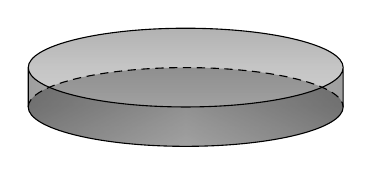
\begin{tikzpicture}
\fill[top color=gray!50!black,bottom color=gray!10,middle color=gray,shading=axis,opacity=0.25] (0,0) circle (2cm and 0.5cm);
\fill[left color=gray!50!black,right color=gray!50!black,middle color=gray!50,shading=axis,opacity=0.25] (2,0) -- (2,0.5) arc (360:180:2cm and 0.5cm) -- (-2,0) arc (180:360:2cm and 0.5cm);
\fill[top color=gray!90!,bottom color=gray!2,middle color=gray!30,shading=axis,opacity=0.25] (0,0.5) circle (2cm and 0.5cm);
\draw (-2,0.5) -- (-2,0) arc (180:360:2cm and 0.5cm) -- (2,0.5) ++ (-2,0) circle (2cm and 0.5cm);
\draw[densely dashed] (-2,0) arc (180:0:2cm and 0.5cm);
\end{tikzpicture}
\]


Using the fact that the disk is uniform, so mass density $\sigma$ is uniform
\[
M = \int \rho (\mathbf{x}) d\mathbf{x} = \int \rho(\mathbf{s}) d\mathbf{s} = \sigma \int r d\theta dr = \sigma \frac{1}{2} R^2 2\pi = \sigma \pi R^2
\]
\[
\sigma = \frac{M}{\pi R^2} = \text{ mass per unit area }
\]

\begin{equation}
I  = \int r^2 dm = \int r^2 \sigma r d\theta dr = \sigma \frac{1}{4} r^4 2\pi = \boxed{ \frac{MR^2}{2} }
\end{equation}

\end{enumerate}


\subsection{Euler's equations of motion, Euler's rotation equations}

In the body frame, inertia tensor $J \equiv I$ is time-independent.

\[
\begin{gathered}
\frac{d}{dt} \widehat{\Omega} - \text{ad}^*_{\widehat{\Omega}} \widehat{\Omega} = 0 
\end{gathered}
\]

Use (Eq. (4.36) Kambe (2009) \cite{dgdt:TKambe2009}

\section{Waves}

\subsection{Signals, Fourier Analysis}

See Ch. 10 "Signals and Fourier Anaylsis" of Georgi (1992) \cite{dgdt:Geor1992}.

\subsubsection{Example: A pulse on a String}

See 10.1.1 "A Pulse on a String", Sec. 10.1 "Signals in Forced Oscillation" of Georgi (1992) \cite{dgdt:Geor1992}.

Consider transvere oscillation of a semiinfinite string stretched from $x=0$ to $x=\infty$, driven at $x=0$ with some arbitrary transverse signal $f(t)$, with a boundary condition at $\infty$ that there's no incoming traveling waves.

If given dispersion relation (10.1) of Georgi (1992) \cite{dgdt:Geor1992}
\begin{equation}\label{dgdt:Eq:NondispersiveDispersionRelation}
	\omega^2 = v^2 k^2
\end{equation}
This implies system that satisfies wave equation
\begin{equation}\label{dgdt:Eq:NondispersiveWaveEquation}
	\frac{\partial^2}{\partial t^2} \psi(x,t) = v^2 \frac{\partial^2}{\partial x^2} \psi(x,t)
\end{equation}
((10.2) of Georgi (1992) \cite{dgdt:Geor1992})

Its a mathematical fact that the general solution to Eq. \ref{dgdt:Eq:NondispersiveWaveEquation} 
\begin{equation}
	\psi(x,t) = g(x- vt) + h(x+vt)
\end{equation}
where $g,h $ arbitrary. This fact is because of this straightforward derivation:

\[
\begin{aligned}
& \frac{\partial^2}{ \partial t^2} \psi(x,t) = v^2 (g''(x-vt) + h''(x+vt)) \\
&	\frac{\partial^2}{ \partial x^2} \psi(x,t) = g''(x-vt) + h''(x+vt)
\end{aligned}
\]

Boundary condition at $\infty$ implies $h=0$, because $h$ function describes wave moving in $-x$ direction. EY: by going to infinity, by physical intuition, we don't expect a reflection back from infinity.

Boundary condition at $x=0$ (substitute $x=0$ into $g$ and thus for $\psi$):
\begin{equation}
	g(-vt) = \psi(0,t) = f(t)
\end{equation}
((10.6) of Georgi (1992) \cite{dgdt:Geor1992})

EY: Consider $\tau = t- \frac{x}{v}$:
\[
\begin{aligned}
	& g(-v\tau) = g(x-vt) \\
	& f(\tau) = f(t-\frac{x}{v})
\end{aligned}
\]

Thus we guess that 
\begin{equation}
	\psi(x,t) = f(t- \frac{x}{v})
\end{equation}
((10.7) of Georgi (1992) \cite{dgdt:Geor1992})

e.g. 

\begin{equation}
	f(t) = \begin{cases} 1 - |t| & \text{ for } |t| \leq 1 \\
		0 & \text{for } |t| >1 \end{cases}
\end{equation}
((10.8) of Georgi (1992) \cite{dgdt:Geor1992})

\subsubsection{Introduction to Fourier integrals}

The idea is to use linearity in a clever way. \\
We can take $f(t)$ apart into its component angular frequencies. \\
We already know how to solve forced oscillatio nproblem for each angular frequency. \\
\begin{itemize}
	\item Take individual solutions and add them back up. 
	\item The advantage of this is that it works for any dispersion relation, not just for Eq. \ref{dgdt:Eq:NondispersiveDispersionRelation}.
\end{itemize}

\begin{equation}\label{dgdt:Eq:FourierIntegral}
	f(t) = \int_{-\infty}^{\infty} d\omega C(\omega) e^{-i\omega t}
\end{equation}
((10.9) of Georgi (1992) \cite{dgdt:Geor1992})

\begin{theorem}[Properties of Fourier integrals, coefficients]
In Eq. \ref{dgdt:Eq:FourierIntegral}
\begin{equation}
	C(\omega) = C(-\omega)^*
\end{equation}
\end{theorem}

\begin{proof}
If $f(t) \in \mathbb{R}$, $f(t) = f^*(t)$ and so
\[
\begin{gathered}
	f(t) = \int_{-\infty}^{\infty} d\omega C(\omega) e^{-i\omega t} = f(t)^* = \int_{-\infty}^{\infty} d(\omega) C^*(\omega) e^{i\omega t} = \int_{\infty}^{-\infty} d(-\omega) C(-\omega)^* e^{-i\omega t} = \int_{-\infty}^{\infty} d(\omega) C(-\omega)^* e^{-i\omega t} \\
	\Longrightarrow C(\omega) = C(-\omega)^*
\end{gathered}
\]
\end{proof}

Since each frequency component of the force produces a wave traveling in $+x$ direction, we use linear superposition, and so we have
\[
\Longrightarrow \psi(x,t) = \int_{-\infty}^{\infty} d\omega C(\omega) e^{-i\omega t + ikx}
\]

\subsubsection{Dispersive Media, Group Velocity}

See 10.2.1 "Group Velocity", Sec. 10.2 "Dispersive Media and Group Velocity" of Georgi (1992) \cite{dgdt:Geor1992}.

\subsubsection{Group Velocity}

You can send signals in a dispersive medium; the trick is to send the signal not directly as the function, $f(t)$, but as modulation of harmonic signal,
\begin{equation}
	f(t) = f_s(t) \cos{\omega_0 t}
\end{equation}
((10.17) of Georgi (1992) \cite{dgdt:Geor1992}), where $f_s(t)$ is the signal. Very often, you want to do this anyway because the important frequencies in your signal, \\
$f_s(t)$, \\
may not match frequencies of the waves with which you want to send the signal, $\omega_0$ of $\cos{\omega_0 t}$. \\

Example: AM radio transmission, in which signal is derived from sound with a typical frequency of a few hundred cycles per second (Hz), but is carried as a modulation of amplitude of an electromagnetic radio wave, with frequency of a few million cycles per second ($\omega_0$).

Consider 
\[
\cos{ (k_+ x - \omega_+ t)} + \cos{ (k_- x - \omega_- t)} \equiv c(k_+ x - \omega_+ t) + c(k_- x - \omega_- t)
\]
Let $k_{\pm} = k_0 \pm k_s$, $\omega_{\pm} = \omega_0 \pm \omega_s$ for $k_s \ll k_0$, $\omega_s \ll \omega_0$.

Then
\begin{equation}\label{dgdt:Eq:Example2TravelingWavesWithCarrierFrequency}
\begin{gathered}
	c(k_{\pm} x - \omega_{\pm}t) = c(k_{\pm} x) c(\omega_{\pm}t) + s(k_{\pm} x) s(\omega_{\pm} t) 
\end{gathered}
\end{equation}
and so for each term,
\[
\begin{gathered}
\begin{gathered}
	c(k_{\pm} x) c(\omega_{\pm} t) = c((k_0 \pm k_s) x) c((\omega_0 \pm \omega_s) t) = (c(k_0x) c(k_s x) \mp s(k_0x) s(k_s x)) (c(\omega_0 t) c(\omega_s t) \mp s(\omega_0 t) s(\omega_0 t)) = \\
= c(k_s x) c(\omega_s t)c(k_0x) c(\omega_0 t) \mp c(k_s x) s(\omega_s t) c(k_0 x) s(\omega_0t) \mp s(k_sx) c(\omega_s t) s(k_0x) c(\omega_0 t) + s(k_s x) s(\omega_s t) s(k_0x ) s(\omega_0 t) 
\end{gathered} \\
\quad \quad \\
\begin{gathered}
	s(k_{\pm}x) s(\omega_{\pm} t) = s(k_0 \pm k_s)x s(\omega_0 \pm \omega_s) t = (s(k_0x) c(k_sx) \pm c(k_0x) s(k_sx) ) (s (\omega_0 t) c(\omega_s t) \pm c(\omega_0 t) s(\omega_s t) ) = \\
	= c(k_s x) c(\omega_s t) s(k_0 x) s(\omega_0 t) \pm c(k_s x) s(\omega_s t) s(k_0x) c(\omega_0 t) \pm s(k_s x) s(\omega_0 t) c(k_0x) s(\omega_0 t) + s(k_s x) s(\omega_s t) c(k_0x) c(\omega_0 t)
\end{gathered}
\end{gathered}
\]
Terms with $\pm$ or $\mp$ in front cancel for when considering the total expression summing 2 terms in Eq. \ref{dgdt:Eq:Example2TravelingWavesWithCarrierFrequency}, and so
\begin{equation}\label{dgdt:Eq:SignalAndCarrierWavesAs2TravelingWaves}
\begin{gathered}
	\Longrightarrow 2 \cdot \left[ c(k_sx) c(\omega_s t) (c(k_0x - \omega_0t)) + s(k_s x) s(\omega_s t) c(k_0x - \omega_0t) \right] = 2 c(k_s x - \omega_s t) c(k_0x - \omega_0 t)
\end{gathered}
\end{equation}
((10.21) of Georgi (1992) \cite{dgdt:Geor1992})

Since $k_s \ll k_0$, and $\omega_s \ll \omega_0$, so $c(k_s x - \omega_s t)$ varies slowly in $x$ and $t$ compared to second factor. You should think of this first factor as the signal in Eq. \ref{dgdt:Eq:SignalAndCarrierWavesAs2TravelingWaves}. The second factor is called the \textbf{carrier wave}.

Then Eq. \ref{dgdt:Eq:SignalAndCarrierWavesAs2TravelingWaves} describes a signal that moves with velocity
\begin{equation}
	v_s = \frac{ \omega_s }{k_s } = \frac{ \omega_+ - \omega_- }{ k_+ - k_- }
\end{equation}
((10.22) of Georgi (1992) \cite{dgdt:Geor1992}) while smaller waves associated with second factor, carrier wave, move with velocity 
\begin{equation}
	v_0 = \frac{\omega_0}{k_0}
\end{equation}
((10.23) of Georgi (1992) \cite{dgdt:Geor1992})

In limit as $k_+ - k_- = 2k_s$ becomes small, $v_s \equiv \frac{\omega_+ - \omega_- }{ k_+ - k_-} \mapsto \left. \frac{\partial \omega}{\partial k} \right|_{k=k_0}$.

$v_g = \left. \frac{\partial \omega}{ \partial k} \right|_{k=k_0}$ is called the "group velocity"; measures the speed the signal can actually be sent.

Suppose dispersion relation is slowly varying for some range of frequencies near some frequency $\omega_0$, 
\[
\begin{gathered}
	\omega = \omega(k) = \omega_0 + (k- k_0) \left. \frac{ \partial \omega}{ \partial k } \right|_{k=k_0} + \dots \\
	\omega_0 \equiv \omega(k_0)
\end{gathered}
\]
Higher order terms negligible only if $\Delta \omega \ll \omega_0$. If so let 
\[
\begin{gathered}
	\begin{gathered}
		\omega = vk + a \\
		k = \frac{\omega}{v} + b
	\end{gathered} \text{ \quad \, since \quad \, } \begin{gathered}
	a = \omega_0 - k_v \\
	b = -\frac{a}{v} = k_0 - \frac{ \omega_0}{v}
\end{gathered}
\end{gathered}
\]

$v$ is group velocity, $\left. v = \frac{\partial \omega}{ \partial k} \right|_{k=k_0}$

Send signal of form $f(t) e^{-i\omega_0 t}$ (modulate the amplitude by $f(t)$ that's non-zero for some range of frequencies, of carrier wave $e^{-i \omega_0 t}$):
\[
\begin{gathered}
	\psi(0,t) = f(t) e^{-i \omega_0 t} = \int_{-\infty}^{\infty} d\omega C(\omega) e^{-i\omega t} e^{-i\omega_0 t} = \int_{-\infty}^{\infty} d\omega C(\omega) e^{-i(\omega + \omega_0)t} = \int_{-\infty}^{\infty} d\omega C(\omega - \omega_0) e^{-i\omega t}
\end{gathered}
\]
where we used linearity or i.e. linear superposition or i.e. adding up frequency components for second equality, and $u= \omega + \omega_0$ substitution for 3rd equality.

Thus
\[
\psi(x,t) = \int_{-\infty}^{\infty} d\omega C(\omega - \omega_0) e^{-i\omega t} e^{ikx}
\]

For approximation $k = \frac{\omega }{v} + b$, 
\[
\begin{gathered}
\psi(x,t) = \int_{-\infty}^{\infty} d\omega C(\omega - \omega_0) e^{-i\omega t} e^{ i \left( \frac{\omega x}{v} + bx \right) } = \int_{-\infty}^{\infty} d\omega C(\omega - \omega_0) e^{ -i \omega \left( t - \frac{x}{v} \right) } e^{ibx } = \\
= \int_{-\infty}^{\infty} d\omega C(\omega) e^{-i (\omega + \omega_0) \left( t - \frac{x}{v} \right) } e^{ibx} = f(t - \frac{x}{v})	 e^{-i \omega_0 (t - \frac{x}{v} ) + ibx}
\end{gathered}
\]

Thus, for signal $f(t)$ s.t. $C(\omega) \approx 0$ for $| \omega - \omega_0| > \Delta \omega$, where $\Delta \omega \ll \omega_0$, \\
modulation $f(t)$ travels without change of shape at group velocity $v = \left. \frac{ \partial \omega}{ \partial k } \right|_{k=k_0}$. \\
Phase velocity $v_{\phi} = \frac{\omega}{k}$ has nothing to do with transmission of information, but notice because of $e^{ibx} = \exp{ \left( i \left( k_0 - \frac{ \omega_0}{v} \right) \right) }$ carrier wave travels at phase velocity
\[
\begin{gathered}
	\frac{ \omega_0 }{ b + \frac{\omega_0}{v} } = \frac{ \omega_0}{ k_0 - \frac{\omega_0}{v} + \frac{\omega_0}{v} } = \frac{\omega_0}{k_0} = v_{\phi}
\end{gathered}
\]

"You can see the difference between phase velocity and group velocity in your pool or bathtub by making a wave packet consisting of severla shorter waves." pp. 232, Sec. 10.2 of Georgi (1992) \cite{dgdt:Geor1992}).

\subsubsection{Bandwidth, Fidelity, Uncertainty}

See Sec. 10.3 "Bandwidth, Fidelity, and Uncertainty" of Georgi (1992) \cite{dgdt:Geor1992}.

\subsubsection{Inverse Fourier Transform}

Now suppose we have the inverse Fourier transform to be of this form:
\begin{equation}\label{dgdt:Eq:InverseFourierTransform}
C(\omega) = \frac{1}{ 2\pi} \int_{-\infty}^{\infty} dt f(t) e^{i\omega t}
\end{equation}

Recall $f(t) = \int_{-\infty}^{\infty} d\omega C(\omega) e^{-i\omega t}$ of Eq. \ref{dgdt:Eq:FourierIntegral}. 

Given $\frac{1}{2\pi}\int_{-\infty}^{\infty} dt f(t) e^{i\omega t}$ of Eq. \ref{dgdt:Eq:InverseFourierTransform}, insert Eq. \ref{dgdt:Eq:FourierIntegral} for $f(t)$:
\[
\begin{gathered}
	\frac{1}{2\pi} \int_{-\infty}^{\infty}dt \int_{-\infty}^{\infty} d\omega' C(\omega') e^{i (\omega- \omega')t} = \frac{1}{2\pi} \int_{-\infty}^{\infty} d\omega' C(\omega') \int_{-\infty}^{\infty} dt e^{i (\omega - \omega') t} 
\end{gathered}
\]
$\int_{-\infty}^{\infty} e^{ i(\omega - \omega') t} $ averages to zero unless $\omega' = \omega$.

Therefore $\frac{1}{2\pi} \int_{-\infty}^{\infty} dt f(t) e^{i\omega t} $ is proportional to $C(\omega)$.

Now consider $f(t) = e^{-\Gamma|t|}$.

\[
\begin{gathered}
	\int_{-\infty}^{\infty} dt e^{-\Gamma|t|} e^{i\omega t} =\int_0^{\infty} dt e^{t(i\omega - \Gamma)} + \int_{-\infty}^0 dt e^{i(i\omega + \Gamma) } = \left. \frac{ e^{t(i\omega - \Gamma)} }{ i\omega - \Gamma} \right|_0^{\infty} + \left. \frac{ e^{t(i\omega + \Gamma)} }{ i\omega + \Gamma} \right|_{-\infty}^0 = \frac{ i\omega + \Gamma}{ \omega^2 + \Gamma^2} + \frac{-i\omega + \Gamma}{ \omega^2 +\Gamma^2} = \frac{2\Gamma}{ \omega^2 + \Gamma^2}
\end{gathered}
\]
Note that for $\frac{1}{ i\omega - \Gamma}$, $\frac{1}{ i\omega + \Gamma}$, if $\omega = \mp i\Gamma$, there's a pole; otherwise $\forall \, \omega \in \mathbb{R}$, integral is well-behaved.

Then for this particular case $C(\omega) = \frac{1}{2\pi} \frac{ 2\Gamma}{ \omega^2 + \Gamma^2}$.

For $f(t) = e^{-\Gamma |t|}$, $f(0) = 1$. Then
\[
\int_{-\infty}^{\infty} d\omega C(\omega) e^{-i\omega t} = \int_{-\infty}^{\infty} d\omega \frac{1}{\pi} \frac{ \Gamma e^{-i\omega t} }{ \omega^2 + \Gamma^2} = \frac{1}{\pi} \int_{-\infty}^{\infty} \frac{d\omega \Gamma}{ \omega^2 + \Gamma^2} = \frac{1}{ \pi} \int_{-\pi/2}^{\pi/2} \frac{ \Gamma \sec^2{\theta} d\theta \Gamma}{ \Gamma^2 (\tan^2{\theta} + 1) } = 1
\]
So $\frac{1}{2\pi}$ factor is obtained.

In another way to get $C(\omega)$, the inverse Fourier transform, as the limit of a Fourier waves, consider $\psi(-\pi l,t) = \psi(\pi l,t) $, periodic boundary condition (notice the period is $2\pi l = T$), 
\[
\xrightarrow{ \text{ in general } } \psi(x) = \sum_{j=-\infty}^{\infty} c_j e^{-ijx/l}
\]
Notice that changing $c_j e^{-ijx/l}$ by $2\pi l$ just changes the phase of the exponential by some multiple of $2\pi$ and so each factor indeed obeys the periodic boundary condition.

Likewise, for $f(t)$, s.t. $f(-\pi T) = f(\pi T)$, $T$ large
\[
\begin{aligned}
	& f(t) = \sum_{j=-\infty}^{\infty} c_j e^{-ijt/T} \quad \quad \, \text{ (Fourier transform in time ) } \\
	& c_j = \frac{1}{2\pi T} \int_{-\pi T}^{\pi T} dt e^{ijt/T} f(t) 
\end{aligned}
\]

$\lim_{t\to \infty} f(t) = 0$, then $c_j \to 0$ as $T \to \infty$.  $\Longrightarrow \begin{aligned}
	& c_j T \to C(\omega) \\
	& j/T \to \omega 
\end{aligned}$, so then
\[
f(t) = \sum c_j e^{-ij t/T} = \sum (c_j T) e^{-ijt/T} \frac{1}{T} \to \int_{-\infty}^{\infty} d\omega C(\omega) e^{-i \omega t} 
\]
So we have these important results:
\begin{align}
	& \boxed{ f(t)  = \int_{-\infty}^{\infty} C(\omega) e^{- i\omega t}  }\\
	& \boxed{ C(\omega)  = \frac{1}{2\pi} \int_{-\infty}^{\infty} dt f(t) e^{ i \omega t}  }
\end{align}


\section{Fluid Mechanics, Fluid Flow}

\subsubsection{Courses to consider}

\href{https://ocw.mit.edu/courses/aeronautics-and-astronautics/16-01-unified-engineering-i-ii-iii-iv-fall-2005-spring-2006/fluid-mechanics/}{MIT 16.01, 16.02}

\subsubsection{Videos to watch}

\href{https://youtu.be/pAuQ4Hj2ZrU}{Engineering MAE 130A. Intro to Fluid Mechanics. Lecture 01.} UCI. Follow the rest of the videos.


\subsection{Buoyancy}

From Problem 1.3 of the Japan Physics Olympiad (2014) \cite{dgdt:Japa2014}, Ch. 1, General Physics, Elementary Problems.

\problemhead{1.3} The part of the iceberg above the sea.
\[
\begin{aligned}
& \rho_{sw} = 1024 \, \text{kg}/m^3 \\
& \rho_{ice} = 917 \, \text{kg}/m^3
\end{aligned}
\]
with $sw \equiv$ sea water.

Find the ratio of the volume of the part of the iceberg above the sea to whole volume of the iceberg.

\solutionhead{1.3}

\textbf{The buoyancy force exerted on the iceberg is equal to the weight of the seawater displaced by the iceberg}.

\[
\begin{gathered}
	\rho_{sw} g V_{is} = \rho_{ice} gV_{ice} \Longrightarrow \frac{ \rho_{sw} }{ \rho_{ice}} = \frac{V_{ice}}{ V_{is}} 
\end{gathered}
\]
with iceberg in sea $\equiv$ is.

iceberg above sea $\equiv$ as
\[
\begin{gathered}
V_{as} / V_{ice} = \frac{V_{ice} - V_{is}}{ V_{ice}} = 1 - \frac{V_{is}}{V_{ice}} = 1 - \frac{ \rho_{ice}}{ \rho_{sw}} = 1 - \frac{917 \, \text{kg}/m^3}{ 1024 \, \text{kg}/ m^3 } = \frac{ 1024 - 917 }{ 1024} = \frac{107 } {1024} 
\end{gathered}
\]

\textbf{The buoyancy on a body equals the resultant force due to the pressure exerted by the surrounding fluid}, i.e.
\textbf{The buoyancy force exerted on a body (iceberg) is equal to the resultant force due to pressure exerted by the surrounding fluid (seawater)}.


Pressure on body of volume $V$ due to its surrounding fluid (whose density is $\rho$) acts perpendicularly to the boundary surface between the body and the fluid. 

Since fluid pressure at a deep location is greater than that at shallow location, resultant force due to pressure on boundary surface points upward. This resultant force is the buoyancy, $F$, acting on body. 

Consider region of fluid with same volume $V$ as body. \\

buoyancy $F \equiv$ force exerted vertically on body by its surrounding fluid $ \underbrace{ =}_{ \text{ balance gravitational force acting on} V }  \rho g V$ \\

For a body floating in a fluid, the magnitude of the buoyancy force acting on the body is equal to the magnitude of the gravitational force on the fluid displaced by the part of the body submerged in the fluid.



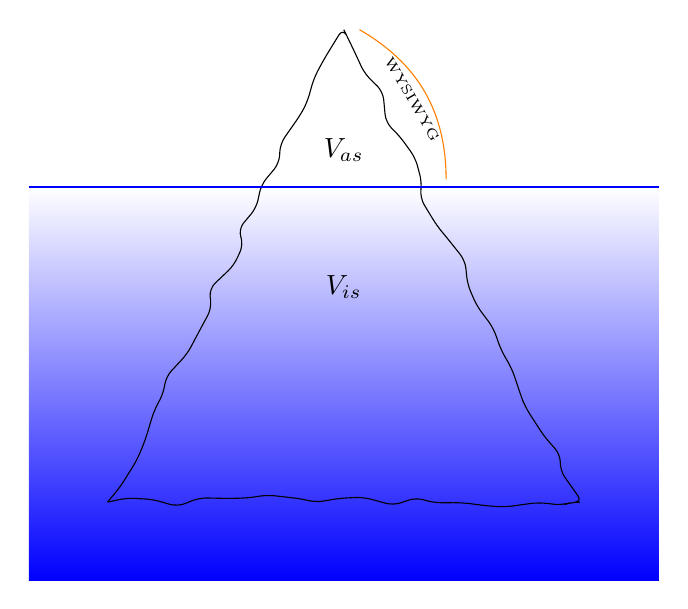
\begin{tikzpicture}
\fill [shade,
        top color=white,
        bottom color=blue] (-4,0) rectangle (4,-5);
\draw [decoration={random steps,segment length=0.3cm,amplitude=.1cm},
        decorate,
        rounded corners=.1cm]
     (-3,-4) -- (3,-4) -- (0,2) -- (-3,-4);
\draw [thick,blue] (-4,0) -- (4,0);
\node [above=2mm] at (0,0) {$V_{as}$};
\node [below=1cm] at (0,0) {$V_{is}$};
\draw [orange] (0.2,2) to[bend left] node[pos=0.5,sloped,below,font=\tiny,black] {WYSIWYG} (1.3,0.1);
\end{tikzpicture}

\subsection{Fluids as a State of Matter}

cf. Pert (2013) \cite{dgdt:Pert2013}, Ch. 1 Introduction, 1.1 Fluids as a State of Matter.

fluid - isotropic, (no directional preference; identical values of a property in all directions), \\
locally homogeneous, macroscopic material, \\
whose particles are free to move within constraints established by the dynamical laws of continuum physics. \\
\emph{requirement that fluid be a continuum} - if volume of fluid successively subdivided into smaller elements, each element will remain structurally similar to its parent, and this subdivision can be carried out down to infinitesimal volumes. \\

\textbf{fluid particle} - fictitious particle fixed within fluid continuum and moving with flow velocity; \\
represents average over large number of microscopic particles. \\

\textbf{fluid point} - fixed in fluid moving with flow velocity; \\
- fluid particle always situated at same fluid point. \\

\textbf{infinitesimal volume} - within continuum of fluid, large compared with microscopic scales, but small compared with macroscopic ones. \\

fluid is made up of discrete microscopic particles, namely molecules, distributed randomly, with \\
distribution of velocities characteristic of fluid in termal equilibrium, typically Maxwell-Boltzmann distribution in a gas. \\

At typical experimental densities, \\
intermolecular separation extremely small and very much less than lab scale, i.e. $l_s \ll L_0$ \\
possible to average over small volumes which contain very large number of particles, yet very small on lab scale, $N-V$ in $V_0$, $V_0^{1/3} \ll L_0$ \\
$\Longrightarrow$ allow us to recover continuum approximation \\
obtain terms which characterize fluid as bulk material \\

Typical average quantities: \\
Density, $\rho$: number of mass particles per unit volume. \\
temperature, $\tau$: average energy of random motion per particle in thermal equilibrium \\
pressure $p$ average momentum flow associated with random motion per unit area. \\
flow velocity $u$ - mean velocity of molecules averaging out random motion. \\

role of collisions amongst particles important in defining irreversibility through loss of correlation between particles. \\

\emph{mean free path} $l_0$ - particles collide on average after distance equal to $l_0$ and time after collision interval\\

since fluid mechanics assumes fluid particles in thermal equilibrium and randomly distributed, this condition requires that spatial and temporal averages be taken to include large number of collisions; i.e. lab scale length $L_0$ large compared with $l_0$, and time to collision interval \\

effects of collisions on fluid transport (momentum and energy) are averaged over thermal distribution to yield bulk properties of material, namely viscosity and thermal conduction, respectively. \\

theory: flow of basic fluid may be calculated using Newtonian mechanics, classical thermodynamics, viscosity and thermal conductivity values. \\
Conditions under which this theory may be applied: \\
\begin{itemize}
	\item lab-scale lengths $L_0$ must be large compared with intermolecule separation and mean free path $l_0$ 
	\item characteristic lab times $T_0$ must be large compared with collision interval
	\item fluid locally in thermal equilibrium
\end{itemize}

cf. 1.2 The Fundamental Equations for Flows of a Dissipationless Fluid. Pert (2013) \cite{dgdt:Pert2013}

\textbf{inviscid limit} - viscosity and thermal conduction are neglected \\
\textbf{adiabatic flow} - specific entropy of fluid particle constant in time \\
\textbf{isentropic flow} - specific entropy of each fluid particle has same initial value \\

many flows are both isentropic and adiabatic, e.g. ideal steady fluid flow, whose specific entropy an entry is everywhere constant.

\emph{Eulerian frame} - lab frame, coordinates fixed in space and time, derivatives are usual partial derivatives
\[
\left. \frac{ \partial }{ \partial t} \right|_{\mathbf{r}}, \, \left. \nabla \right|_t
\]
Consider coordinate system $(t, x^1, x^2, x^3)$ and so each vector field $\mathbf{e}_j$ forming basis of tangent space at each pt. expressed as linear combination of coordinate vector fields
\[
\left. \frac{\partial}{\partial t} \right|_{\mathbf{r}}, \, \left. \frac{\partial}{\partial x^1} \right|_{t}, \, \left. \frac{\partial}{\partial x^2} \right|_{t}, \, \left. \frac{\partial}{\partial x^3} \right|_{t},
\]

in Lagrangian frame, spatial variation seen by particle due to its motion is absorbed into time derivative:
\[
\frac{d}{dt} = \frac{\partial }{ \partial t} + \mathbf{v} \cdot \mathbf{\nabla} 
\]

Rather, consider total time derivative of integral of $n$-form: 
\[
\frac{d}{dt} \int_{V_0} \omega = \int_{V_0} \mathcal{L}_{\frac{\partial}{\partial t} + \mathbf{v} } \omega 
\]

Volume form $\Omega^n(M) = \bigwedge^n (T^*M)$
\[
\text{vol}^n \in \Gamma(\Omega^n(M)) = \Gamma(\bigwedge^n T^*M)
\]
i.e. $\text{vol}^n$ is $n$-form, a section of the line bundle, $\Omega^n(M) = \bigwedge^n T^*M$

Now
\[
\text{vol}^n = \frac{\sqrt{g}}{ n!} \epsilon_{i_1, \dots i_n} dx^{i_1} \wedge \dots \wedge dx^{i_n}
\]

Consider 
\[
\text{vol}^{n+1} = \frac{\sqrt{g}}{ (n+1)!} \epsilon_{i_0 i_1, \dots i_n} dx^{i_0} \wedge dx^{i_1} \wedge \dots \wedge dx^{i_n}
\]

\subsection{Lagrangian frame}

cf. Pert (2013) \cite{dgdt:Pert2013} 1.3 Lagrangian Frame.

\textbf{Lagrangian frame} - frame of the moving particle; \\
Lagrangian reference frame considers fluid from point of view of an observer on a fluid particle. \\

fluid particle may be conveniently identified by coordinate set, which is fixed on the particle, \\
$\mathbf{\Lambda} = (\lambda, \mu, \nu)$ i.e. triad of numbers. \\
e.g. $\mathbf{\Lambda}$ maybe initial position of particle $\mathbf{r}_0 = (x_0, y_0, z_0)$, i.e. fluid particle labeled by some (time-independent) vector field $\mathbf{x}_0 \equiv \mathbf{\Lambda}$. \\

$\Longrightarrow $ position, velocity, thermodynamic state of particles are therefore functions of time alone. \\
$\Longrightarrow$ leads to simple set of kinematic and dynamic relations governing motion of particle \\
\[
\begin{gathered}
	\mathbf{r} = \mathbf{r}(t) = (x(t), y(t), z(t)) = (x^1(t), x^2(t), x^3(t)) \\ 
	\dot{ \mathbf{r}} \equiv \dot{\mathbf{r}}(t) \equiv \frac{d\mathbf{r}}{dt} \equiv \frac{d\mathbf{r}}{dt} (t) = \mathbf{v} \equiv \mathbf{v}(t)
\end{gathered}
\]
or 
\begin{equation}
\begin{gathered}
\frac{d\mathbf{r}}{dt} = \mathbf{v} \\ 
\frac{d\mathbf{v}}{dt} = \frac{\mathbf{F}}{m}
\end{gathered}
\end{equation}
cf. Eq. (1.2) of Pert (2013) \cite{dgdt:Pert2013}, i.e. \\

flow described by function $\mathbf{X}(\mathbf{x}_0, t)$ giving position of particle labeled at $\mathbf{x}_0$ at time $t$.

\subsection{Momentum conservation in Lagrangian Frame-Euler's Equation}

Recall that a connection $\nabla$ on smooth manifold $(M, \mathcal{O}, \mathcal{A})$ is a map that takes a pair consisting of a vector (field) $X$ and $(p,q)$-tensor field $T$ and sends them to a $(p,q)-$ tensor (field) $\nabla_XT$, i.e. 
\[
\nabla : \mathfrak{X}(M) \times (\otimes^p TM \otimes^q T^*M) \to \otimes^p TM \otimes^q T^*M
\]
s.t. 
\[
\begin{aligned}
& \nabla_X f = Xf \quad \, \forall \, f \in C^{\infty}(M) \\ 
& \nabla_X(T + S) = \nabla_X T + \nabla_X S \\ 
& \nabla_X(T(\omega, Y)) = (\nabla_X T)(\omega, T) + T(\nabla_X \omega, Y) + T(\omega, \nabla_X Y) \\
& \nabla_{fX + Z} T = f\nabla_X T + \nabla_Z T , \quad \, f \in C^{\infty}(M) \quad \, \text{ "Leibnitz" rule }
\end{aligned}
\]
cf. Schuller, International Winter School on Gravity and Light held central lectures.

Remember that in the Lagrangian frame, we are an observer following an individual fluid parcel or i.e. "fluid particle" as it moves through space and time. This fluid particle will obey Newton's 2nd. law: $\nabla_{u} u = \frac{F}{m} \Longleftrightarrow m \cdot \mathfrak{a} = F$. 

\[
\begin{gathered}
\nabla_u u = \nabla_{u^{\mu}\frac{\partial}{\partial x^{\mu}}} (u^{\nu} \frac{\partial}{\partial x^{\nu}}) = u^{\mu} \nabla_{\frac{ \partial }{\partial x^{\mu}} } (u^{\nu} \frac{ \partial }{ \partial x^{\nu}}) =  u^{\mu} \left( \nabla_{\frac{ \partial }{\partial x^{\mu}} } u^{\nu} \right) \frac{ \partial }{ \partial x^{\nu}} + u^{\mu} u^{\nu} \nabla_{\frac{ \partial }{\partial x^{\mu}} }  \frac{ \partial }{ \partial x^{\nu}} = \\
	= u^{\mu} \frac{ \partial u^{\nu} }{ \partial x^{\mu}} \frac{\partial}{\partial x^{\nu}} + u^{\mu}u^{\nu} \Gamma^{\gamma}_{\mu \nu} \frac{\partial}{\partial x^{\gamma}}
	\end{gathered}
	\]

Let $u^0 = 1$.
\[
\begin{gathered}
\nabla_u u = \frac{\partial u^a}{\partial t} \frac{\partial }{ \partial x^a} + u^b \frac{\partial u^a}{\partial x^b} \frac{\partial}{\partial x^a} + u^{\mu} u^{\nu} \Gamma^a_{\mu \nu} \frac{\partial}{\partial x^a}
\end{gathered}
\]
where $\Gamma^0_{ba} = 0$ since $\nabla dt =0$ and we choose a stratified atlas $\mathcal{A}_{\text{stratified}}$.

Then let
\[
\int \rho \text{vol}^n \nabla_u u = F_{\text{tot}}  = \int f^i \text{vol}^n \otimes e_i
\]

From Sec. 2.4 Equations of Motion Neglecting Viscosity, pp. 38, Sabersky, et. al. (1998) \cite{dgdt:SAHG1998}, the principal forces are those due to pressures acting on surfaces and to forces acting directly on a mass of the particle:
\[
\begin{gathered}
\int_{\partial V} p dS^i \otimes e_i = \int_V \mathbf{d} (pdS^i \otimes e_i) = \int_V \frac{\partial p}{\partial x^j} dx^j \wedge \left( \frac{\sqrt{g}}{(n-1)!} \epsilon^i_{\, i_2, \dots i_n} dx^{i_2} \wedge \dots \wedge dx^{i_n} \right) \otimes e_i = \\
\int_V \frac{\partial p}{\partial x^j} g^{ij} \text{vol}^n \otimes e_i = \int_V (\text{grad}p)^i \text{vol}^n \otimes e_i \\
\Longrightarrow \int \rho \text{vol}^n \nabla_u u = -\int_V (\text{grad}p)^i \text{vol}^n \otimes e_i + \int_V f^i \text{vol}^n \otimes e_i
\end{gathered}
\]
\begin{equation}\label{dgdt:Eq:EulerianEquationMomentumConservationFluidFlow}
\begin{gathered}
\Longrightarrow \rho (\nabla_u u)^i = -(\text{grad}p)^i + f^i \\
(\nabla_u u)^i = -\frac{1}{\rho} (\text{grad}p)^i + f^i
\end{gathered}
\end{equation}
describes the motion of a perfect fluid.

Assuming a non-rotating, inertial frame (so that we can set the Christoffel symbols to 0),
\begin{equation}\label{dgdt:Eq:EulerianEquationMomentumConservationFluidFlowInertialFrame}
\frac{\partial}{\partial t} u^i + u^b \frac{\partial u^i}{\partial x^b} = - \frac{1}{\rho}(\text{grad}p)^i + f^i
\end{equation}
which describes the motion of the perfect fluid in an inertial ref. frame. Compare this to Eqns. (2.10a- 2.10c) of Sabersky (1998) \cite{dgdt:SAHG1998}. Sabersky says that no assumptions were made about density so these results apply to compressible fluid as well as incompressible ones. Also Eqns. \ref{dgdt:Eq:EulerianEquationMomentumConservationFluidFlow}, \ref{dgdt:Eq:EulerianEquationMomentumConservationFluidFlowInertialFrame} are called either Euler's Equation by Pert (2013) \cite{dgdt:Pert2013} or Eulerian equation by Sabersky, et. al. (1998) \cite{dgdt:SAHG1998}



\subsection{Mass Conservation for Fluid Flow, Continuum media}

The mass of fluid in some volume $V_0 \subset N$ is $\int_{V^0} \rho \text{vol}^n$, where $\rho$ is fluid density, $\rho \in C^{\infty}(N)$.  

The total mass of fluid flowing out of volume $V_0$ is 
\[
\begin{gathered}
\frac{d}{dt} \int_{V_0} \rho \text{vol}^n = \int_{V_0} \mathcal{L}_{\frac{\partial}{\partial t} + \textbf{u}} (\rho \text{vol}^n) = \int_{V_0} \frac{ \partial }{\partial t} \rho \text{vol}^n + \int_{V_0} \mathcal{L}_u \rho \text{vol}^n   \\
\int_{V_0} \mathcal{L}_u \rho \text{vol}^n = \int_{V_0} di_{\mathbf{u}} \rho \text{vol}^n  + i_{\mathbf{u}} d\rho \text{vol}^n = \int_{V_0} di_{\mathbf{u}} \rho \text{vol}^n + 0 = \int_{V_0} di_{\mathbf{u}} \rho \text{vol}^n = \int_{\partial V_0} i_{\mathbf{u}} \rho \text{vol}^n
\end{gathered}
\]  
Now
\[
\begin{gathered}
i_u \text{vol}^n = i_u\frac{\sqrt{g}}{n!} \epsilon_{i_1 \dots i_n} dx^{i_1} \wedge \dots \wedge dx^{i_n} \\ 
i_u dx^{i_1} \wedge \dots \wedge dx^{i_n} = u^{i_1} dx^{i_2} \wedge \dots \wedge dx^{i_n} - dx^{i_1} \wedge u^{i_2} dx^{i_3} \wedge \dots \wedge dx^{i_n} +  \dots + (-1)^{n+1} dx^{i_1} \wedge \dots \wedge dx^{i_{n-1}} u^{i_n} = \epsilon^{i_1 \dots i_n}_{j_1 \dots j_n } u^{j_1 } dx^{j_2} \wedge \dots \wedge dx^{j_n}  
\end{gathered} 
\]
\begin{equation}\label{dgdt:Eq:TimeIndependentMassVolumeTerm}
\Longrightarrow i_u\text{vol}^n = \frac{ \sqrt{g}}{ (n-1)!} \epsilon_{j_1 \dots j_n} u^{j_1} dx^{j_2} \wedge \dots \wedge dx^{j_n}
\end{equation}

We can also rewrite Eq. \ref{dgdt:Eq:TimeIndependentMassVolumeTerm} to be a "surface differential":
\begin{equation}
\begin{gathered}
\int_{V_0} \mathbf{d}i_{\mathbf{u}} \rho \text{vol}^n = \int_{\partial V_0} i_{\mathbf{u}} \rho \text{vol}^n = \\
\int_{\partial V_0} \rho \frac{ \sqrt{g}}{ (n-1)!} u^{j_1} \epsilon_{j_1 j_2 \dots j_n} dx^{j_2} \wedge \dots \wedge dx^{j_n} \equiv \int_{\partial V_0} \rho \mathbf{u} \cdot d\mathbf{S} \equiv \int_{\partial V_0} \rho \langle \mathbf{u}, d\mathbf{S} \rangle 
\end{gathered}
\end{equation}


If $\sqrt{g} = 1$, $n=2$, 
\[
i_u \text{vol}^2 = (u^1 dx^2 - u^2 dx^1) = u\cdot n_1 dx^2 + u\cdot n_2 dx^1 = u\cdot n dS
\]
with $n_1 =e_1$ and $n_2=-e_2$.  

Now 
\[
\begin{gathered}
di_u \rho \text{vol}^n = \\
= \frac{ \partial ( \sqrt{g} \rho u^{j_1} ) }{ \partial x^k} \frac{ \epsilon_{j_1 \dots j_n} }{ (n-1)! } dx^k \wedge dx^{j_2} \wedge \dots \wedge dx^{j_n} = \frac{ \partial (\sqrt{ g} \rho u^k) }{ \partial x^k} \frac{ \epsilon_{j_1 \dots j_n }}{ n!} dx^{j_1} \wedge \dots \wedge dx^{j_n} = \frac{1}{\sqrt{g}} \frac{ \partial (\sqrt{g} \rho u^k)}{ \partial x^k} \text{vol}^n = \\
= \frac{ \partial (\rho u^k)}{ \partial x^k} \text{vol}^n + \rho u^k \frac{ \partial \ln{ \sqrt{g}}}{ \partial x^k} \text{vol}^n = \text{div}(\rho u) \text{vol}^n + \rho u^k \frac{ \partial \ln{ \sqrt{g}}}{ \partial x^k} \text{vol}^n
\end{gathered}
\]
Now if $\sqrt{g}=1$, then 
\[
\begin{gathered}
\frac{d}{dt} \int_{V_0} \rho \text{vol}^n = \int_{V_0} \frac{ \partial \rho }{ \partial t} \text{vol}^n + \int_{V_0} di_u \rho \text{vol}^n = \int_{V_0} \frac{ \partial \rho }{ \partial t} \text{vol}^n + \int_{V_0} \text{div}(\rho u) \text{vol}^n \Longrightarrow \frac{ \partial \rho}{\partial t} + \text{div}(\rho u) = 0
\end{gathered}
\]
which is the so-called mass continuity equation.  $ j = \rho u$ is the mass flux density.  

Thus,

\begin{equation}\label{dgdt:Eq:MassConservationForContinuum}
\begin{gathered}
\text{(mass conservation)} \\
m = m(t) := \int_{V_0} \rho \text{vol}^n, \, V_0 \subset N \\
\dot{m} \equiv \frac{d}{dt}m(t) = \int_{V_0} \left( \frac{\partial \rho }{ \partial t} \text{vol}^n + \mathbf{d}i_{\mathbf{u}} \rho \text{vol}^n \right) = \boxed{ \int_{V_0} \frac{ \partial \rho }{ \partial t} \text{vol}^n + \int_{\partial V_0} \rho \mathbf{u} \cdot d\mathbf{S} } \\
\text{ if } \sqrt{g} = 1, \text{ and } \dot{m} = 0, \text{ then } \\
\frac{\partial \rho }{ \partial t} + \text{div}(\rho \mathbf{u}) = 0 
\end{gathered}
\end{equation}

Sec. 1.4 Eulerian Frame, 1.4.1 Conservation of Mass-Equation of Continuity, pp. 8 of Pert (2013) \cite{dgdt:Pert2013} says that Eq. \ref{dgdt:Eq:MassConservationForContinuum} is for the Eulerian Frame.

From \href{https://en.wikipedia.org/wiki/Lagrangian_and_Eulerian_specification_of_the_flow_field}{wikipedia}, recall that the \emph{Eulerian specification} focuses on specific locations in space through which fluid flow as time passes. Visualize by sitting on bank of river and watch water pass fixed location. In the Eulerian specification of field, field represented as a function of position $\mathbf{x}$, time $t$, e.g. $\mathbf{u}(\mathbf{x}, t) \equiv $ flow velocity.




TODO: 20190804 Frankel (2012) \cite{dgdt:TFrankel2012} in pp. 138 and onwards, for Sec. 4.3. Differentiation of Integrals posed the rightful question, "How does one compute the rate of change of an integral when the domain of integration is also changing?" Revisit the derivation from a Lie derivative and 1-parameter flow point of view.

Force should not be represented by a vector but rather by a 1-form. Then, 
\[
f \in \Omega^1(N), \, f=f(t, \mathbf{x}) = f_j dx^j \, \, j=1, \dots n , \, \mathbf{x} = (x^1, \dots x^n), \, \text{dim}N = n
\]
Indeed, the reason for $f$ to be a 1-form is that we integrate differential forms, we don't integrate vectors. 

\begin{equation}
W = \int_C f \qquad \, \text{(line integral)}
\end{equation}

\emph{If} $f$ conservative, $\exists\, $ scalar $U = U(x)$; $x\in N$ s.t. $f=-dU$.

Let $\mathbf{u} = u^j(t,\mathbf{x}) \frac{\partial}{ \partial x^j} \in \mathfrak{X}(N)$ generate flow $\phi_t$.

The Lie derivative along vector field $\mathbf{u}$, $\mathcal{L}_{\mathbf{u}}$, can be calculated in at least 2 ways: from the definition:
\[
\mathcal{L}_{\mathbf{u}} \omega  =\frac{d}{dt} \left. \right|_{t = 0} \phi_t^*\omega
\]
or Cartan's magic formula:
\begin{equation}
\begin{gathered}
	\mathcal{L}_{\mathbf{u}} \text{vol}^n = (i_{\mathbf{u}}\mathbf{d} + \mathbf{d}i_{\mathbf{u}}) \text{vol}^n = 0 + \mathbf{d}i_{\mathbf{u}} \text{vol}^n = \mathbf{d}i_{\mathbf{u}} \left( \frac{ \sqrt{g}}{n!} \epsilon_{i_1 \dots i_n} dx^{i_1} \wedge \dots \wedge dx^{i_n} \right) = \\ 
	= \mathbf{d} \left( \frac{\sqrt{g}}{(n-1)! } \epsilon_{j_1 \dots j_n} u^{j_1} dx^{j_2} \wedge \dots \wedge dx^{j_n} \right) = \frac{ \partial (\sqrt{g} u^{j_1} )}{ \partial x^k} \frac{ \epsilon_{j_1 \dots j_n}}{(n-1)!} dx^k \wedge dx^{j_2} \wedge \dots \wedge dx^{j_n} = \\
	= \frac{ \partial (\sqrt{g} u^{j_1}) }{ \partial x^k} \frac{ \epsilon_{j_1 \dots j_n} }{ (n-1)! } \epsilon^{k j_2 \dots j_n}_{ k_1, \dots, k_n} dx^{k_1} \wedge \dots \wedge dx^{k_n} \underbrace{\left( \frac{ \sqrt{g}}{ \sqrt{g}} \right)}_{=1} = \frac{1}{\sqrt{g}} \frac{ \partial ( \sqrt{g} u^k) }{ \partial x^k} \text{vol}^n =  \\
	= (\text{div}{\mathbf{u}}) \text{vol}^n
\end{gathered}
\end{equation}
cf. \url{https://math.stackexchange.com/questions/2566381/lie-derivative-of-volume-form?rq=1}

Note that
\[
\begin{gathered}
	\text{div}: \mathfrak{X}(N) \to C^{\infty}(N) \\ 
 \mathcal{L}_{\mathbf{u}}: \Omega^n(N) \to \Omega^n(N) 
\end{gathered}
\]

Frankel (2012) \cite{dgdt:TFrankel2012} on pp. lvii of the "Elasticity and Stresses" section offered this analogy: "While work in particle mechanics pairs a force covector ($f_i$) with a contravariant tangent vector ($dx^i/dt$) to a curve, work done by traction in elasticity pairs the contravariant stress force 2-form $\mathcal{S}$ with the covector valued deformation 1-form $\mathcal{E}$, to yield a scalar valued 3-form.

Instead of pushing along a curve (line) particle to do work, what does it mean to do work on a moving fluid element? One could possibly try to consider the deformation of a volume element under fluid flow. Frankel (2012) \cite{dgdt:TFrankel2012} in Sec. 4.2. The Lie Derivative of a Form, on pp. 132, asks "If a flow deforms some attribute, say volume, how does one measure the deformation? $\mathcal{L}_{\mathbf{u}}\text{vol}^n$ "is the $n$-form that reads off the rate of change of volume of a parallelopiped spanned by $n$ vectors that are pushed forward by the flow $\phi_t$." So, "in other words, $\mathcal{L}_{\mathbf{u}}\text{vol}^n$ \emph{measures how volumes are changing under the flow} $\phi_t$ \emph{generated by} $\mathbf{X}$" on pp. 133 on Frankel (2012) \cite{dgdt:TFrankel2012}. 

Then rate of work done on a fluid element could be the following:

\[
\begin{gathered}
W = \int_V \mathcal{L}_{\mathbf{u}}(p \text{vol}^n) = \int_V \mathbf{d} i_{\mathbf{u}} p \text{vol}^n = \int_{\partial V} i_{\mathbf{u}} p \text{vol}^n = \int_{\partial V} p \mathbf{u} \cdot d\mathbf{S} 
\end{gathered}
\]

TODO: work on a fluid element?

\subsection{Bernoulli's equation}

\subsubsection{Simple cases}

cf. Ch. 3 The Bernoulli Equation, Sec. 3.2 "A Simple Form of the Bernoulli Equation", pp. 90, Sabersky, et. al. (1998) \cite{dgdt:SAHG1998}


Start from Eq. \ref{dgdt:Eq:EulerianEquationMomentumConservationFluidFlow}. So
\[
(\nabla_u u)^i = \frac{-1}{\rho} (\text{grad}p)^i + f^i
\]
Suppose $f^i=0$ (no external forces), $\frac{\partial u^i}{\partial t} = 0$ (steady flow). Suppose $\Gamma^a_{\mu \nu} =0$ (Cartesian coordinates? TODO: find out the conditions when this is true).

Suppose the flow is irrotational (TODO: find out the condition for irrotational flow; is it when having streamlines or ?). For the curl, recall that an external derivative $\mathbf{d}$ takes a 1-form into a 2-form. So consider
\[
\begin{gathered}
 \mathbf{u} \in \mathfrak{X}(V), \mathbf{u} \xrightarrow{\flat} u_i dx^i = g_{ij} u^j dx^i \\ 
 d\mathbf{u}^{\flat} \in \Omega^2(V), \, \mathbf{d}\mathbf{u}^{\flat} = \frac{\partial u_j}{\partial x^i} dx^i \wedge dx^j = \frac{ \partial (g_{ij} u^j) }{\partial x^a} dx^a \wedge dx^i
\end{gathered}
\]
If we have the condition that the flow is irrotational, i.e. 
\begin{equation}
\mathbf{d}\mathbf{u}^{\flat} = 0
\end{equation}
then
\[
\begin{gathered}
	\mathbf{d}\mathbf{u}^{\flat} (\mathbf{u}) = \frac{\partial (u_i) }{ \partial x^a} u^a dx^i - \frac{\partial (u_i) }{ \partial x^a} dx^a u^i = 0 \Longrightarrow u^a \frac{ \partial (u_i) }{ \partial x^a} dx^i = u^i \frac{\partial u_i}{ \partial x^a} dx^a
\end{gathered}
\]







Take the exterior derivative $\mathbf{d}$ of the inner product of a vector with itself in the most general case on a metric manifold:
\[
\begin{gathered}
d(u_i u^i) = d(g_{ij} u^j u^i) = \frac{ \partial g_{ij} }{ \partial x^k} u^j u^i dx^k  + g_{ij} \frac{ \partial u^j}{ \partial x^k} u^i dx^k + g_{ij} u^j \frac{\partial u^i}{\partial x^k} dx^k = \\
= 2 u_j \frac{ \partial u^j}{\partial x^k} dx^k + u^i u^j \frac{\partial g_{ij}}{\partial x^k} dx^k 
\end{gathered}
\]


Since the Christoffel symbols are the connection coefficients of a \emph{metric-compatible} affine connection (i.e. they can be used to construct a connection $\nabla$ s.t. $\nabla g = 0$), then \footnote{ \href{https://physics.stackexchange.com/questions/175235/prove-christoffel-symbol-identity}{"Prove Christoffel Symbol Identity", Physics StackExchange}}

\begin{equation}
\nabla_i g_{jk} = \frac{ \partial g_{jk}}{\partial x^i} - \Gamma^s_{ji} g_{sk} - \Gamma^s_{ki} g_{js} = 0
\end{equation}
and so
\begin{equation}
\begin{gathered}
 u^i u^j \frac{ \partial g_{ij}}{\partial x^k} = u^i u^j \left[ \Gamma^s_{ik} g_{sj} + \Gamma^s_{jk} g_{is} \right] = u^i u_s \Gamma^s_{ik} + u_s u^j \Gamma^s_{jk} = 2u_s u^i \Gamma^s_{ik}
\end{gathered}
\end{equation}



Then 
\begin{equation}\label{dgdt:Eq:ExteriorDerivativeOfMagnitudeSquareOfVector}
\begin{gathered}
\frac{1}{2} \mathbf{d}(u^2) = u_j \frac{ \partial u^j}{\partial x^k} dx^k + u_s u^i \Gamma^s_{ik} dx^k
\end{gathered}
\end{equation}

Eq. \ref{dgdt:Eq:ExteriorDerivativeOfMagnitudeSquareOfVector} only depended upon the fact that the connection $\nabla$ is \emph{metric-compatible}.

So if we suppose that the Christoffel symbols $\Gamma^s_{ik}$ are 0, and have irrotational flow, as well,
\[
\begin{gathered}
\mathbf{d}(u^2 / 2) = u_j \frac{\partial u^j}{ \partial x^k} dx^k  + 0 = u^a \frac{ \partial u_i}{\partial x^a} dx^i 
\end{gathered}
\]

Now consider the RHS of Eq. \ref{dgdt:Eq:EulerianEquationMomentumConservationFluidFlow}, with $f_i =0$,
\[
\begin{gathered}
	\frac{-1}{\rho} (\text{grad}{p})^i \xrightarrow{ \flat} \frac{-1}{\rho} (\text{grad}p)^i g_{ij} dx^j = \frac{-1}{\rho}  \frac{\partial p}{\partial x^k} g^{ki} g_{ij} dx^j = \frac{-1}{\rho} \frac{ \partial p}{\partial x^j} dx^j = \frac{-1}{\rho} \mathbf{d}p
\end{gathered}
\]
So if the fluid is incompressible, then $\rho$ is constant and so we can write

\begin{equation}
\mathbf{d} \left( \frac{u^2}{2} + \frac{p}{\rho} \right) = 0 
\end{equation}
for any irrotational, incompressible, fluid flow with no (external) body forces.

\subsubsection{Venturi tube example}

cf. Example 3.1 in Sabersky, et. al. (1998) \cite{dgdt:SAHG1998}

Consider flow of liquid through the tube shown. Determine pressure difference between points 1 and 2 as a function of flow rate $Q$, density $\rho$. Velocity assumed constant over cross sections, and pressure will also be assumed uniform over each of these 2 areas $A_1$, $A_2$. Also assume there's no viscosity. 

\solutionhead{Example 3.1 in Sabersky, et. al. (1998) \cite{dgdt:SAHG1998}}

Since density is constant, continuity equation requires that for $Q$ the volume flow rate,
\[
\text{flow rate} Q = u_1 A_1 = u_2 A_2
\]

\[
\begin{gathered}
	\frac{u_1^2}{2} + \frac{p_1}{\rho_1} = \frac{u_2^2}{2} + \frac{p_2}{\rho_2} \Longrightarrow \begin{aligned} & \quad \\ 
	& \frac{Q^2}{2A_1^2} + - \frac{Q^2}{2A_2^2} = \frac{ -(p_1- p_2) }{\rho}  \\
	& \frac{Q^2}{2} \left( \frac{1}{A_1^2} - \frac{1}{A_2^2} \right) = \frac{-(p_1 - p_2) }{\rho} \end{aligned} \text{ or } 
p_1 - p_2 = \frac{ + \rho Q^2}{2A_2^2} \left( 1 - \frac{A_2^2}{A_1^2} \right) 
\end{gathered}
\]

\subsubsection{Conservative body forces with Bernoulli equation}

cf. Sec. 3.3 in Sabersky, et. al. (1998) \cite{dgdt:SAHG1998}

Consider $U= U(x)$, force potential. 

\[
\begin{gathered}
	-\mathbf{d}U = \frac{ - \partial U}{\partial x^i} dx^i = f_i dx^i \\
 \mathbf{d}\left( \frac{u^2}{2} + \frac{p}{\rho} + U \right) = 0 
\end{gathered}
\]

\subsubsection{Barotropic Fluids ($\rho = \rho(p)$) with Bernoulli equation}

cf. Sec. 3.4 in Sabersky, et. al. (1998) \cite{dgdt:SAHG1998}

\emph{Barotropic fluid}: density is single-valued function of $p$. In the absence of heat transfer and absence of entropy change, by thermodynamics this can be shown to be barotropic.

\[
\begin{gathered}
\mathbf{d} \left( \frac{u^2}{2} \right) = -\frac{1}{\rho} \mathbf{d}p - \mathbf{d}U \text{ or } \mathbf{d} \left( \frac{u^2}{2} + U \right) + \frac{1}{\rho} \mathbf{d}p
\end{gathered}
\]

Suppose $i=i(p)$ s.t. $di = \frac{\partial i}{\partial p} dp = \frac{1}{\rho (p)} = \frac{di}{dp} dp$. So
\[
\begin{gathered}
\frac{di}{dp} = \frac{1}{\rho(p)} \text{ or } i = \int \frac{1}{\rho} dp + \text{ const } \\
\Longrightarrow \mathbf{d} \left( \frac{u^2}{2} + U + i \right) = 0 
\end{gathered}
\]

In special case of isentropic flow of perfect gas, $\frac{P}{\rho^{\nu}} = $ const. and $ i =\int \frac{dp}{p^{1/\nu}} = \frac{kp^{1-1/\nu}}{1- 1/\nu} = $ enthalpy.

\subsubsection{Nonsteady flow $\frac{\partial u}{\partial t}$ with Bernoulli equation}

First, use the musical isomorphism to transform the (1,0) tensor:
\[
\begin{gathered}
\frac{ \partial u^i}{\partial t}\frac{\partial}{\partial x^i} \xrightarrow{\flat} g_{ij} \frac{\partial u^i}{\partial t} dx^j
\end{gathered}
\]

Along a curve $\begin{aligned} & \quad \\ 
& \gamma = \gamma^i(t) = x^i(t) \text{ s.t. } \\
& \dot{\gamma} = \dot{\gamma}^i(t) \frac{ \partial}{\partial x^i} = u^i(t, \gamma(t)) \frac{\partial}{\partial x^i}
\end{aligned}$. Then

\[
\begin{gathered}
\int_{\gamma} g_{ij} \frac{\partial u^i}{\partial t} dx^j = \int g_{ij} \frac{\partial u^i}{\partial t} \dot{\gamma}^j(t) dt = \int g_{ij} \frac{\partial u^i}{\partial t} u^j dt = \int \frac{\partial \| u \| }{ \partial t} dt 
\end{gathered}
\]
The last step can be made only if the metric $g$ is time-independent.

cf. Example 3.2 in Sabersky, et. al. (1998) \cite{dgdt:SAHG1998}. 

Consider the \emph{efflux} of liquid of density $\rho$ through an orifice of area $A_0$ at the bottom of a large tank of cross-sectional area $A_t$. \\
The depth of liquid at the given instant is $y$. \\
pressure exerted on the liquid in the tank is maintained at $p_t$, \\
pressure outside the orifice is the atmospheric pressure $p_a$. \\

The action of gravity is to be considered, but frictional effects may be neglected. Velocity of efflux $u_j$ is to be determined for these conditions. \\

efflux - something given off in or as if in a stream (Webster dictionary)

\solutionhead{Example 3.2 in Sabersky, et. al. (1998) \cite{dgdt:SAHG1998}}

In Sec. 3.8(b) flows through orifices discussed in great detail. For this example, \\
assume the orifice is carefully designed so streamlines at orifice exit are parallel and thus orifice area $A_0$ and cross-sectional area of jet $A_j$ are equal there.


cf. Example 3.3 in Sabersky, et. al. (1998) \cite{dgdt:SAHG1998}. Example of a problem in which nonsteady terms cannot be neglected. 

\section{Viscous Fluids, Navier-Stokes Equation Applications}

cf. Ch. 2, Viscous Fluids, Sec. 15. The equations of motions of a viscous fluid, Landau and Lifshitz (1987) \cite{dgdt:LLandauELifshitz1987}

Recall Navier-Stokes equation for \emph{compressible, viscous} fluid flow:

\begin{equation}
\boxed{
\rho \left( \frac{\partial u^i }{ \partial t} + u^j \frac{ \partial u^i }{ \partial x^j } \right) = - \frac{ \partial p }{ \partial x^i } + (\lambda + \mu ) \frac{\partial }{ \partial x^i } \text{div} u + \mu \Delta u^i
}
\end{equation}

Compare this with the expression in Eq. 15.6, Landau and Lifshitz (1987) \cite{dgdt:LLandauELifshitz1987}

\begin{equation}
\begin{gathered}
	\rho \left[ \frac{ \partial \mathbf{v}}{ \partial t } + (\mathbf{v} \cdot \textbf{grad} ) \mathbf{v} \right] = -\textbf{grad} p + \eta \Delta \mathbf{v} + (\zeta + \frac{1}{3} \eta) \textbf{grad} \text{div} \mathbf{v}
\end{gathered}
\end{equation}

$\mu \equiv \eta$, fluid isotropic, so properties described by scalar quantities. \\
$\mu \equiv \eta$ viscosity coefficients, \\
$\lambda + \mu \equiv \zeta + \frac{1}{3} \eta$, $\zeta \equiv $ second viscosity.

\subsection{Flow in a pipe}



\section{Thermodynamics}

\quad \\ 
Let $\Sigma$ be a (topological) manifold. \\
Suppose $U$ is a global coordinate on $\Sigma$:
\begin{equation}
\begin{gathered}
\text{ (First Law of Thermodynamics (energy conservation)) } \\
\boxed{ dU = Q - W \text{ or } Q = dU + W }
\end{gathered}
\end{equation}
where $dU, Q, W \in \Omega^1(\Sigma)$ (i.e. $dU, Q, W$ are 1-forms over manifold $\Sigma$).

\quad \\ 
Consider a path in $\Sigma$, $\gamma$, $\gamma : \mathbb{R} \to \Sigma$, \\
and using a chart $(U, S^1, \dots , S^n)$ (e.g. $n=1$, $S^1 = v$ for volume)
\[
\begin{gathered}
\gamma(t) = (U(t), S^1(t), \dots, S^n(t)) \\
\dot{\gamma} \in \mathfrak{X}(\Sigma), \, \dot{\gamma} = \dot{U} \frac{ \partial }{ \partial U} + \dot{S}^i \frac{ \partial }{ \partial S^i} 
\end{gathered}
\]
Now 
\[
\begin{gathered}
dU(\dot{\gamma}) = \dot{\gamma}(U) = \dot{U} \frac{ \partial }{ \partial U} U + 0 = \dot{U} \\
	Q(\dot{\gamma}) = Q(t) dt\left( \dot{\gamma} \frac{ \partial }{ \partial t} \right) = Q(t) \dot{\gamma} \\ 
	\Longrightarrow \dot{U} = Q(t) \dot{\gamma} - W(t) \dot{\gamma}
\end{gathered}
\]

Recall that for enthalpy $H$, $H := U + pV$, $H=H(\sigma, p)$

TODO 20190804 Derive and check convection form of enthalpy against both Kittle and Kroemer plus thermodynamics and Sonntag, et. al. 

Incomplete:
\[
\begin{gathered} 
dH = Q + Vdp \\
W = pdV = pdV + Vdp - Vdp = d(pV) - Vdp = \\
dE = Q-W + \mu dH \\
dE = Q- W + \widehat{h} dN
\end{gathered} 
\]

$U \to E$ notation is to promote the internal energy $U$ to include kinetic and potential energies, so that possibly, $E = U + \text{K.E.} + \text{P.E.}$, or, i.e., $E$ includes internal energy and mechanical energy.

$G = \mu N$ \\
$G = U - \tau \sigma + pV \xrightarrow{U \to E} G = E-\tau \sigma + pV \Longrightarrow \tau \check{h}$
\[
\begin{gathered}
dE = Q + W + \mu dN = Q + W + (\check{h} - \tau \check{\sigma})dN
\end{gathered}
\]
\[
\begin{gathered}
Q = \tau d\sigma = \tau d(N \check{\sigma}) = \tau N d\check{\sigma} + \tau \check{\sigma} dN
\end{gathered}
\]

\quad \\ 
$\tau N d\check{\sigma}$ is the entropy change due to change in entropy per particle; i.e. \textbf{conduction term} \\
$\tau \check{\sigma} dN$ is entropy change due to change in number of particles, i.e. \textbf{convection term}

\[
\begin{gathered}
dE = Q + W + \check{h} dN - \tau \check{\sigma} dN = \tau N d\check{\sigma} + \tau \check{\sigma} dN + W + \check{h} dN - \tau \check{\sigma} dN = \tau N d\check{\sigma} + W + \check{h} dN
\end{gathered}
\]

$m(t) = MN$

Assume only 1 chemical species:
\[
\begin{gathered}
	\check{Q} := \tau N d\check{\sigma} \qquad \, \widehat{h} := \frac{H}{m} = \frac{H}{MN} \\ 
 \Longrightarrow dE = \check{Q} + W + \check{h} dN \frac{M}{M} = \check{Q} + W + \widehat{h} dm
\end{gathered}
\]

The Gibbs free energy equilibrium is given by, 
\[
dG = \mu dN - \sigma d\tau + V dp
\]

For a throttling valve (don't all valves throttle?) the pressure drop is accounted for by the Gibbs free energy, \emph{not} by an isenthalpy condition. 

